% !TEX TS-program = LuaLaTeX

\documentclass{coderdojo}

\usepackage[lf,sfdefault]{gandhi}

\def\SRC{../resources/docs/Coding_Games_in_Python__DK__2018.pdf}
\def\MUcode{/Users/kmurphy/mu_code/coderdojo_tramore/fruit_ninja_games/}

\newfontfamily{\pygameZeroFont}{Marker Felt}
\def\pygameZero{{\pygameZeroFont Pygame Zero}}

\usepackage{pdflscape}

\usetikzlibrary{decorations,decorations.pathreplacing,decorations.pathmorphing}
\tikzstyle{postit}=[fill=yellow!50,draw,thick,
decorate, drop shadow,
decoration={random steps,segment length=3pt,amplitude=1pt},
text width=4cm, font=\scriptsize]

\worksheet{21}{Fruit Ninja Games --- Code}

\newcommand\contentsitem[2]{
	\item \hyperref[#1]{\color{section}\bfseries #2}
}

\usepackage{wrapfig}
\usepackage{float}

\newcommand\TODO[1]{
\begin{itemize}
\item[\todoSymbol] \color{todo} #1
\end{itemize}}


\newcommand\TEST[1][\bf Test your code!]{
	\centerline{\tikz\node[starburst, fill=yellow, draw=red, line width=2pt,align=center] {#1};}
}

\newcommand\TESTSMALL[2][\bf Test your code!]{
{\tikz[scale=#2]\node[starburst, fill=yellow, draw=red, line width=2pt,align=center] {#1};}
}

\usetikzlibrary{decorations.pathreplacing}

%: DOCUMENT
\begin{document}
\maketitle

\begin{dingautolist}{192} 
\contentsitem{ball}{Basic fruit ninja game}\\
Our starting version of the game consists of an apple that appears at random positions on the screen and the computer prints out  "Good shot!" and draws a new apple when you click on the apple, otherwise prints "You missed!" and ends the game.

\codeonly{title={fruit\_ninja\_basic}}
	{1}{100}{\MUcode}{fruit_niinja_basic.py}  
	
\clearpage

\contentsitem{review}{Code review}

The {\em Coding Games with Python} is very good, but it does do a few things that we can improve on. So before we move on we are going to look at our code and see if we can improve it.

\codeonly{title={fruit\_ninja\_refactored}}
	{1}{100}{\MUcode}{fruit_niinja_refactored.py}  
	
\clearpage

\contentsitem{rectangle}{Adding sounds}

One of the reasons we switched over from turtle graphics to \pygameZero\ is to simplify generating sounds --- both short terms sound effects and long term background music. 

\codeonly{title={fruit\_ninja\_sounds}}
	{1}{100}{\MUcode}{fruit_niinja_sounds.py}  
	
\clearpage

\contentsitem{rectangle}{Keeping score}

Currently the game just prints out a different message whenever you miss or hit a fruit. It would be nicer to keep score so that you can show off your shooting skills.  To do this we will create a new variable called \code{score}.  Also we will add a heads up display (HUD) to show the score and game title.    

\codeonly{title={fruit\_ninja\_score}}
	{1}{100}{\MUcode}{fruit_niinja_score.py}  
	
\clearpage

\contentsitem{rectangle}{Moving targets}

Hitting a stationary object is easy \ldots\ what happens if they are moving?

So we are going to change our fixed position fruit to fruit that is thrown upwards from below the screen and then fall back down due to gravity --- now we will need some physics!

\codeonly{title={fruit\_ninja\_physics}}
	{1}{37}{\MUcode}{fruit_niinja_physics.py}  

\codeonly{title={fruit\_ninja\_physics}}
	{38}{100}{\MUcode}{fruit_niinja_physics.py}  
	

\clearpage
	
\contentsitem{rectangle}{Varying targets} 

We don't just want apples! Lets add other fruit also, after all this is `fruit ninja' not `apple ninja'.

\codeonly{title={fruit\_ninja\_final}}
	{1}{46}{\MUcode}{fruit_niinja_final.py}  
	
\codeonly{title={fruit\_ninja\_final}}
	{47}{100}{\MUcode}{fruit_niinja_final.py}  
	
\clearpage

\end{dingautolist}

\end{document}

\clearpage

%: PAGES
\renewcommand{\baselinestretch}{0.55} 


\newcommand\PAIR[3]{
\begin{landscape}\thispagestyle{empty}\hspace{-1.25cm}
\begin{tikzpicture}
\useasboundingbox (0,0) rectangle (28.1,16.75);

\ifnum#1=0\else
\node[anchor=south west] at (0,0) (L) {\includegraphics[page=#1, scale=0.707,angle=0]{\SRC}};\fi
\ifnum#2=0\else
	\node[anchor=south west] at (L.south east) (R)
	{\includegraphics[page=#2,scale=0.707,angle=0]{\SRC}};
	\fi

\node at ($(L.north east)+(0,0.5)$) {\ding{192} \color{section}\bfseries fruit\_ninja\_basic};
#3
\end{tikzpicture}
\end{landscape}}

\def\GRID#1{
\draw (#1.south west) grid (#1.north east);
\foreach \x in {0,1,...,13} {
	\node at ($(#1.south west) + (\x,0.5) $) {\scriptsize\x}; 
	\node at ($(#1.south west) + (\x,8.5) $) {\scriptsize\x}; 
	\node at ($(#1.south west) + (\x,16.5) $) {\scriptsize\x}; 
}
\foreach \y in {1,...,16} {
	\node at ($(#1.south west) + (0, \y) $) {\scriptsize\y}; 
	\node at ($(#1.south west) + (13, \y) $) {\scriptsize\y}; 
}}


\tikzstyle{textfix}=[fill=white,anchor=south west,inner sep=0pt,outer sep=0pt,font=\textfixFont]

\def\BUTTON#1{\includegraphics[width=12pt]{#1}}

%: PAIR{52}{53}
\PAIR{52}{53}{
	\node[textfix, anchor=north west,text width=6.5cm,text depth=2cm] at ($(R.south west) + (1.7,4.15)$) {{\bf New File}\\ In the  mu-editor, click on the new file button,
	\BUTTON{new}};
	\node[anchor=south west] at ($(R.south west) + (0.5,0)$)
		{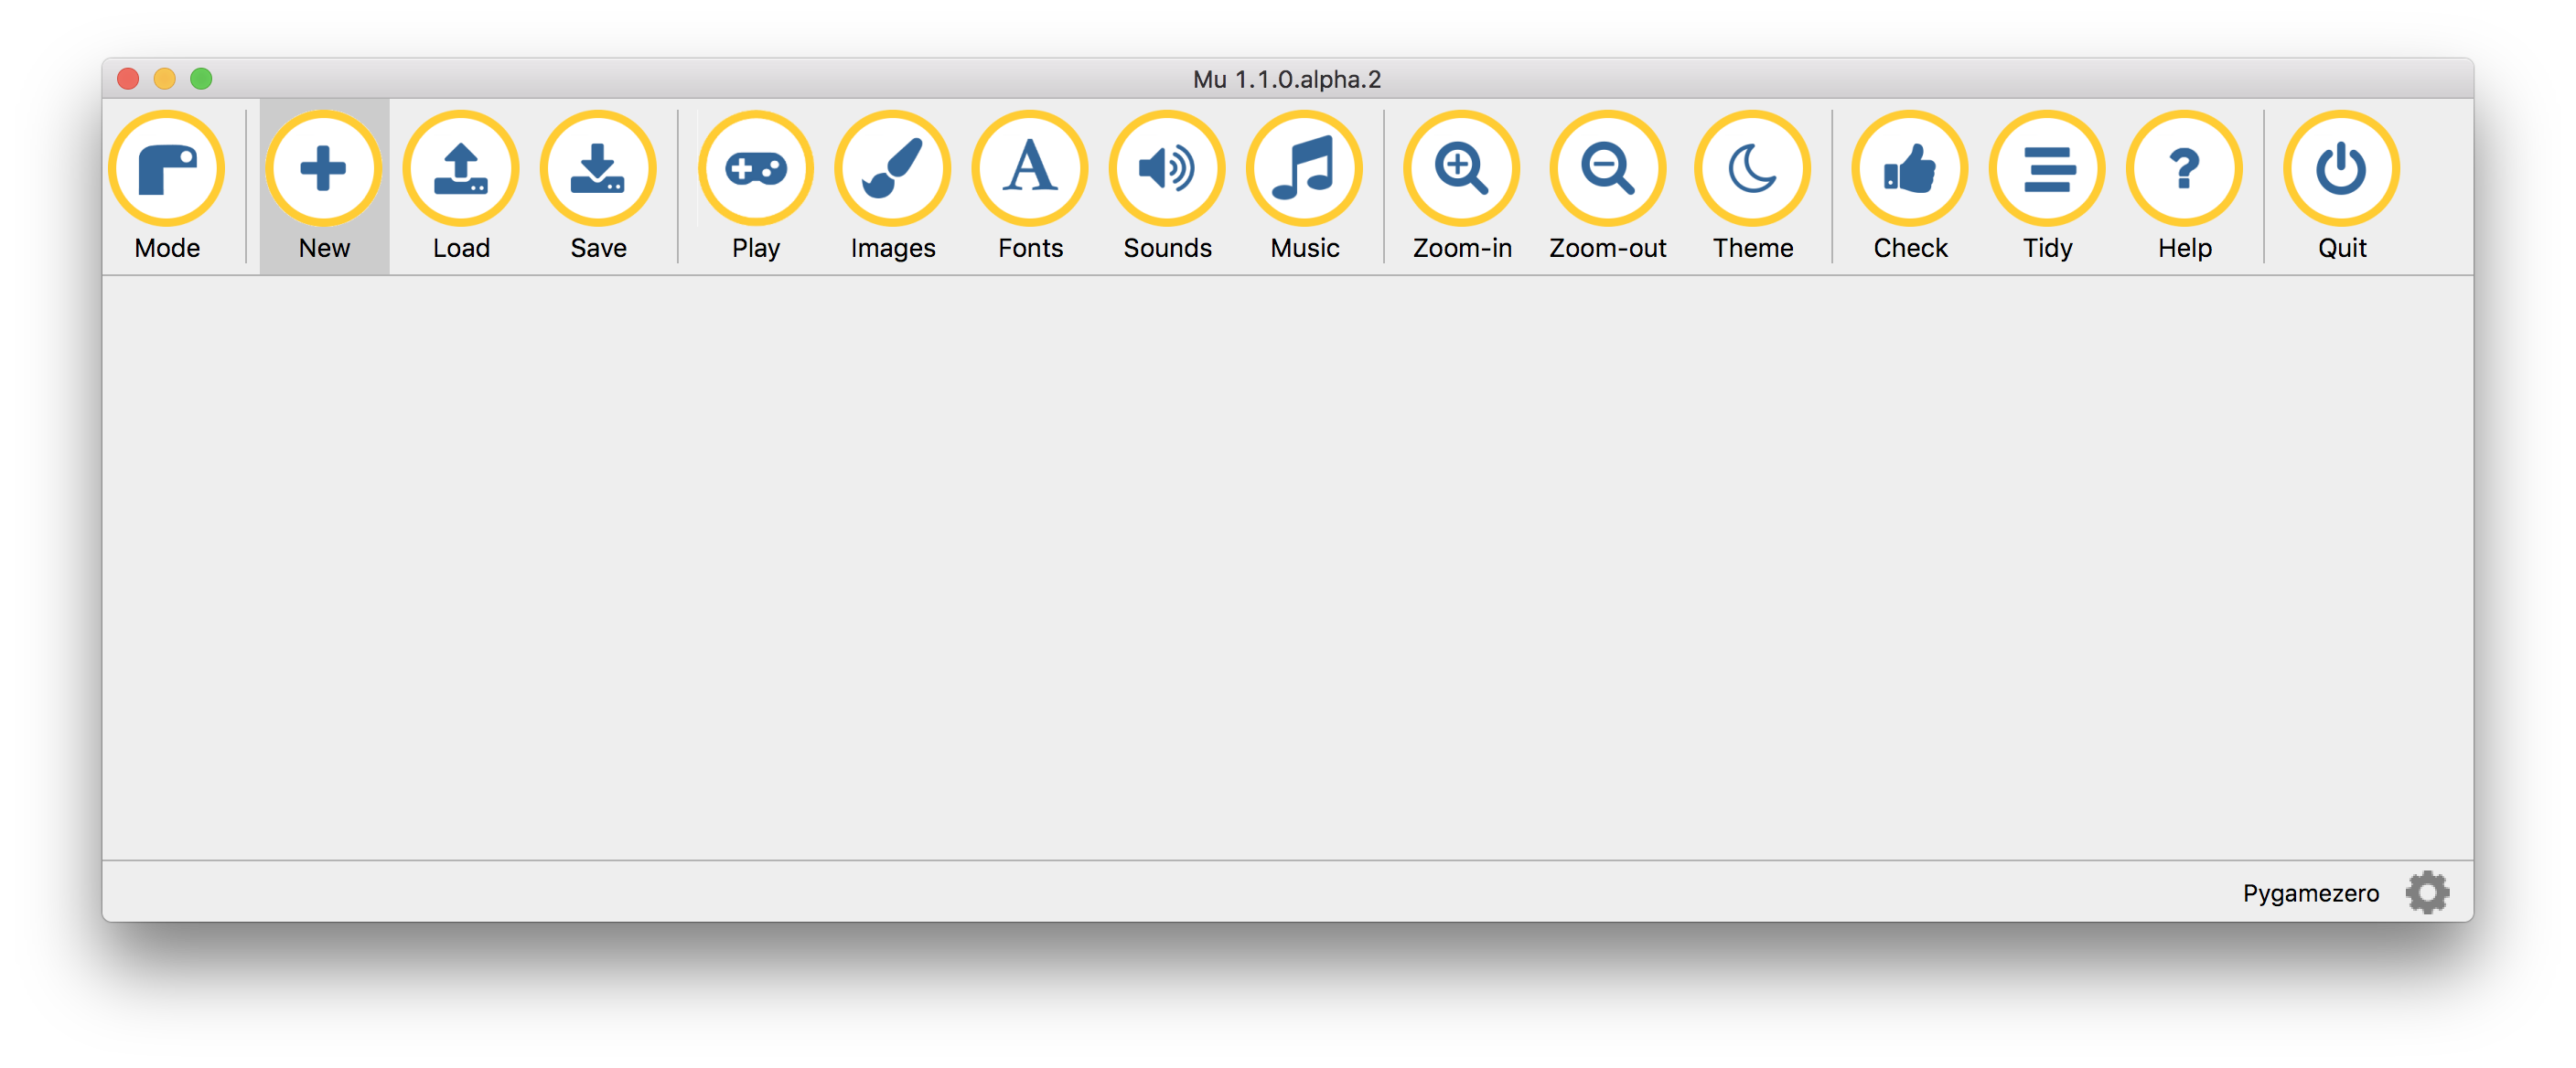
\includegraphics[width=7.5cm]{mu_new}};
}

%: PAIR{54}{55}

\PAIR{54}{55}{
%\GRID{L}\GRID{R}

% step 2
\node[textfix,text width=5.5cm] at ($(L.north west) + (1.65, -1.95)$) 
{{\bfseries Save your game}\\[-6pt]
To save your file click on the save button \BUTTON{save}. Now};
\node[textfix] at ($(L.north west) + (4.25,-2.256)$) {coderdojo\_tramore folder.};
\node[textfix] at ($(L.north west) + (1.32, -3.11)$) {fruit\_ninja\_games};
\node[textfix] at ($(L.north west) + (4.6,-3.11)$) {file as fruit\_ninja\_basic.py};
\node[textfix] at ($(L.north west) + (2.35,-3.74)$) {\smaller fruit\_ninja\_basic.py};
\node[textfix] at ($(L.north west) + (2.65,-4.625)$) {\smaller fruit\_ninja\_games};

% step 3
\node[textfix,text width=6cm,anchor=north west] at ($(L.north west) + (8.3,-1.4)$) {
{\bfseries Set up an image folder}\\
This game uses an image of an apple. Within your
fruit\_ninja\_games folder you want to create a folder called images.\\
Click on the image button \BUTTON{images} and you should see an empty folder where 
you need to put your images.};

\fill[white] ($(L.north west) + (7.38,-3.3)$) rectangle ++(7,-2.2);

% sep 4
\node[textfix,bottom color=gray!25,top color=gray!10] at 
	($(L.north west) + (3.35, -8.625)$) {\smaller fruit\_ninja\_games};
\node[textfix,bottom color=gray!20,top color=gray!20] at 
	($(L.north west) + (1.65, -9.01)$) {\smaller fruit\_ninja\_basic.py};
\draw[-latex] 
	($(L.north west) + (4.6, -6.7)$)
	to [bend left,in=200]
	($(L.north west) + (10.3,-5.4)$) node[above,text width= 4cm] {\smaller I have put a copy of this resource pack in the folder \code{resources}};
	

% step 5
\node[textfix] at 
	($(L.south west) + (9.45, 9.575)$) {\ Mu \ };
	
% step 7
\node[textfix,text width=6cm,anchor=north west] at ($(R.north west) + (8.5,-1.4)$) {
{\bfseries Test your code}\\
To test your code, click on the play button \BUTTON{play}.  \\

To stop, click on the stop button, \BUTTON{stop} \\[12pt]\mbox{}
};

\fill[white] ($(R.north west) + (7.08,-3.3)$) rectangle ++(6,-1.2);

}

%: PAIR{56}{57}
\PAIR{56}{57}{
}

%%: PAIR{58}{59}
%\renewcommand{\baselinestretch}{0.55} 
%\PAIR{58}{0}{
%}

\includegraphics[page=58]{\SRC}

\centerline{\tikz\node[postit,text width=13cm,rotate=2] {
OK, that is our basic game idea, we will now start to add more and more complicated features to it.
};}

\clearpage
\section{Code review}\label{sec:review}

The {\em Coding Games with Python} is very good, but it does do somethings that we can improve on. 

Before we move on we are going to look at our code and see if we can improve it.  We are not trying to change what it does --- that will come later --- instead we want to make the code easier for humans to read and easier for humans to update when they think of something new to add to the game.

So we will make a number of changes:


\TODO{Click on new file icon, \BUTTON{new}, and copy the code from \code{fruit_ninja_basic} into this new file. Save, using icon \BUTTON{save}, as file \code{fruit_ninja_refactored.py}. Finally update the file using the following steps:}

\hspace{-.5cm}
\begin{tikzpicture}
\node[anchor=north west, text width=17cm] at (1,4) (C1) 
	{\ding{192} We set the size of the screen using \code{WIDTH} and \code{HEIGHT} global variables.};
\node[anchor=north west, text width=17cm] at ($(C1.south west)+(0,0.1)$) (C2) 
	{\ding{193} Change name from \code{apple} to \code{fruit} as later we want to deal with more than apples.};
\node[anchor=north west, text width=17cm] at ($(C2.south west)+(0,0.1)$) (C3) 
	{\ding{194} Change name of function \code{place_apple} to \code{place_fruit} as we will use this function to place all fruits.};
\node[anchor=north west, text width=17cm] at ($(C3.south west)+(0,0.1)$) (C4) 
	{\ding{195} Change the limits in function \code{randint} so that the fruit will appear fully on the screen. Now, because we have define global variables \code{WIDTH} and \code{HEIGHT} we can limit the random position of the fruit based on the screen size.};
\node[anchor=north west] at (0,0) (B) {\begin{minipage}{8cm}
\codeonly{listing options={numbers=none}, title={fruit\_ninja\_basic}}
	{1}{6}{\MUcode}{fruit_niinja_basic.py}  
\end{minipage}};

\node[anchor=north west] at (B.north east) (R) {\begin{minipage}{10cm}
\codeonly{listing options={numbers=none}, title={fruit\_ninja\_refactored}}
	{1}{6}{\MUcode}{fruit_niinja_refactored.py}  
\end{minipage}};

\node at ($(R.north west)+(7.5,-1.6)$) {\LARGE \ding{192}};
\draw[line width=2pt,-latex] 
	($(B.north west)+(1,-1.95)$) 
	to[out=335,in=170] 
	node[fill=white] (2) {\LARGE\ding{193}} ($(R.north west)+(0.3,-2.4)$);
\draw[line width=2pt,-latex]  (2) to[out=0,in=170]  ($(R.north west)+(1.3,-4.2)$);
\draw[line width=2pt,-latex]  (2) to[out=0,in=170]  ($(R.north west)+(1.3,-5.5)$);
\draw[line width=2pt,-latex]  (2) to[out=0,in=170]  ($(R.north west)+(1.3,-6.0)$);
\draw[line width=2pt,-latex]  (2) to[out=0,in=170]  ($(R.north west)+(2.1,-7.5)$);

\node at ($(R.north west)+(5.0, -4.6)$) {\LARGE \ding{194}};
\node at ($(R.north west)+(7.5, -5.1)$) {\LARGE \ding{195}};
\end{tikzpicture}


\centerline{\tikz\node[postit,text width=11cm,rotate=-5] {\centerline{\bfseries What is code refactoring?}\\[3pt]
Code refactoring is the process of restructuring existing computer code to improve its readability 
or structure, with the explicit purpose of keeping its meaning or behaviour.\\[3pt]
Refactoring is the part of code maintenance which doesn't fix bugs or add new functionality. Rather it is designed to improve the understandability of the code, to make it easier for human maintenance in the future. \\
};}


\section{Adding sound effects}\label{sec:rectangle}

One of the reasons we switched over from turtle graphics to \pygameZero\ is to simplify generating sounds --- both short term sound effects and long term background music. 

\pygameZero\ treats sound effects and background music separately. 

\subsection{(Short term) Sound effects}

A sound effect is a short (less than a few seconds) audio that is usually played in response to something happening in a game --- target was hit, player died, etc.. To create sound effects you (I have carried out these steps already for you, but list them here so you can try out your own sound effects):

\begin{itemize}
\item \parbox[t]{12cm}{Find a suitable sound effect.  The website
\href{https://www.zapsplat.com}{www.zapsplat.com}, has an excellent search engine and a large collection of free sounds. You need to pay for the WAV format, but the MP3 format is free. I always use the MP3 format.}
\hfill\raisebox{-32pt}[0pt][0pt]{\href{https://www.zapsplat.com}{
\includegraphics[height=30pt]{zap-splat-logo}}}

\vspace{6pt}
{\em\smaller For example, for this game I searched ``target'' and found sound `\href{https://www.zapsplat.com/music/clay-pigeon-shooting-thrower-machine-release-clay-gun-shoots-and-people-cheer-uk-2/}{Clay pigeon shooting, gun shoots and people cheer, UK 2}'. This has a splay sound and a cheer --- I will use both.} 

\item \parbox[t]{13cm}{ 
Convert the sound to WAV format. I use the free audio editor Audacity,
(\href{https://www.audacityteam.org}{www.audacityteam.org}), to edit sound effects and exporting them as MP3 format.}
\hfill\raisebox{-32pt}[0pt][0pt]{\href{https://www.audacityteam.org}{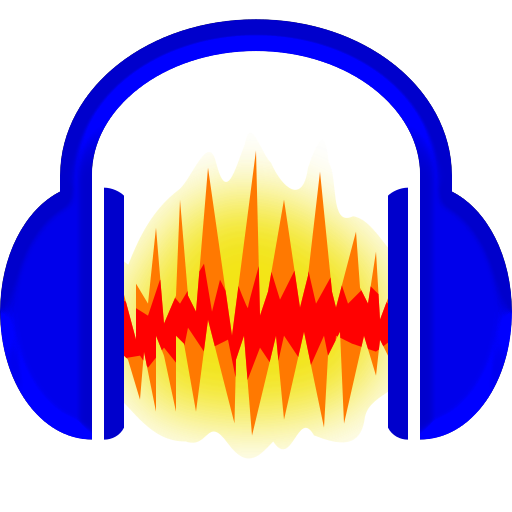
\includegraphics[height=40pt]{audacity}}}

\vspace{6pt}
{\em\smaller For example, using the \href{https://www.zapsplat.com/music/clay-pigeon-shooting-thrower-machine-release-clay-gun-shoots-and-people-cheer-uk-2/}{Clay pigeon shooting, gun shoots and people cheer, UK 2} sound I saved two WAV file --- one contained just the splat sound and the second the splat and cheer sound.
} 

\item 
Copy the sound file into the \code{sounds} sub-folder of \code{fruit_ninja_games}. Make sure that you rename your file so that it uses lower case letters, underscore and numbers only, and that it starts with a letter.

 \vspace{6pt}
{\em\smaller For example, in this game I have two sound effects called 
\code{shoot.wav} and \code{shoot_and_cheer.wav}}

\item
Now wherever in your code you want to play sound, \code{NAME}, you use \code{sounds.NAME.play()}. 

 \vspace{6pt}
{\em\smaller For example, I wanted to play the `\code{shoot}' sound every time the target is hit and on average every ten hits it plays the `\code{shoot_and_cheer}' also so I wrote the following code}

\end{itemize}

\TODO{Click on new file icon, \BUTTON{new}, and copy the code from \code{fruit_ninja_refactored} into this new file. Save, using icon \BUTTON{save}, as file \code{fruit_ninja_sounds.py}. Finally, insert the following code.}

\codeonly{title={}}
	{19}{25}{\MUcode}{fruit_niinja_sounds.py}  



\subsection{(Long term) Background music}

Background music is usually a longer piece of audio and often run in a loop so it repeats until the game is over.
To play background music you:

\begin{itemize}
\item \parbox[t]{11cm}{Find a suitable sound track.  I like the website
\href{https://www.melodyloops.com/music/}{www.melodyloops.com}. It has a good selection of tracks and it has a nice feature of cutting the tracks to whatever length you want and control fade in at the start and fade out at the end of the tracks. }
\hfill\raisebox{-32pt}[0pt][0pt]{\href{https://www.melodyloops.com/music/}{www.melodyloops.com}{
\includegraphics[height=20pt]{melodyloops}}}

 \vspace{6pt}
{\em\smaller For example, for this game I picked The French Lovers Song and set its length to be 90 seconds  with a few second fade out at the end. }

\item
Copy the sound file into the \code{music} sub-folder of \code{fruit_ninja_games}. Make sure that you rename your file so that it uses lower case letters, underscore and numbers only, and that it starts with a letter.

 \vspace{6pt}
{\em\smaller I renamed the downloaded file as \code{the_french_lovers_song.mp3}.}

\item Then to
\begin{itemize}
\item play this track in a loop forever, use code: \code{music.play("the_french_lovers_song")}.
\item play this track once, use code: \code{music.play_once("the_french_lovers_song")}.
\item stop the currently playing track, use code: \code{music.stop()}.
\item pause use code: \code{music.pause()} and to unpause, use code: \code{music.unpause()}.
\item fade out and stop after `duration' seconds, use code: \code{music.fadeout(duration)}.
\item set volume with value in range $0\ldots1$, use code: \code{music.set_volume(volume)}.
\end{itemize}

\end{itemize}


\TODO{Add code to play the \code{the_french_lovers_song} or to play 
\code{trap_ashamaluev_music}  which I found on soundcloud and also downloaded to \code{music} sub-folder.}

\section{Keeping score (and multiple lives)}

\subsection{Keeping score}

Currently the game just prints out a different message whenever you miss or hit a fruit. It would be nicer to keep score so that you can show off your shooting skills.  To do this we will create a new variable called \code{score}.  Also we will add a heads up display (HUD) to show the score and game title. 

\TODO{Click on new file icon, \BUTTON{new}, and copy the code from \code{fruit_ninja_sounds} into this new file. Save, using icon \BUTTON{save}, as file \code{fruit_ninja_score.py}. Finally, update the code as follows.}

\begin{itemize}
\item[{\bf Step 1)}] {\bf Create variables to store the required information.} \\I like to store this information within an actor. So I after creating the actor \code{fruit} I write the following:

\codeonly{listing options={firstline=6,lastline=6,numbers=none}}{6}{6}{\MUcode}{fruit_niinja_score.py}

\item[{\bf Step 2)}] {\bf Update variables when needed.}\\ For the score, we want to increase this by one every time we hit the target, so we have

\codeonly{listing options={firstline=27,lastline=28,numbers=none}}{27}{28}{\MUcode}{fruit_niinja_score.py}

\item[{\bf Step 3)}] {\bf Display information.}\\ 
\begin{minipage}{.6\textwidth}
For all our games, I'm going to display the score on the top left, the game name in the centre, and lives (or other information) on the top right. So the screen looks like this.
\end{minipage}
\hfill
\begin{minipage}{.39\textwidth}\centering
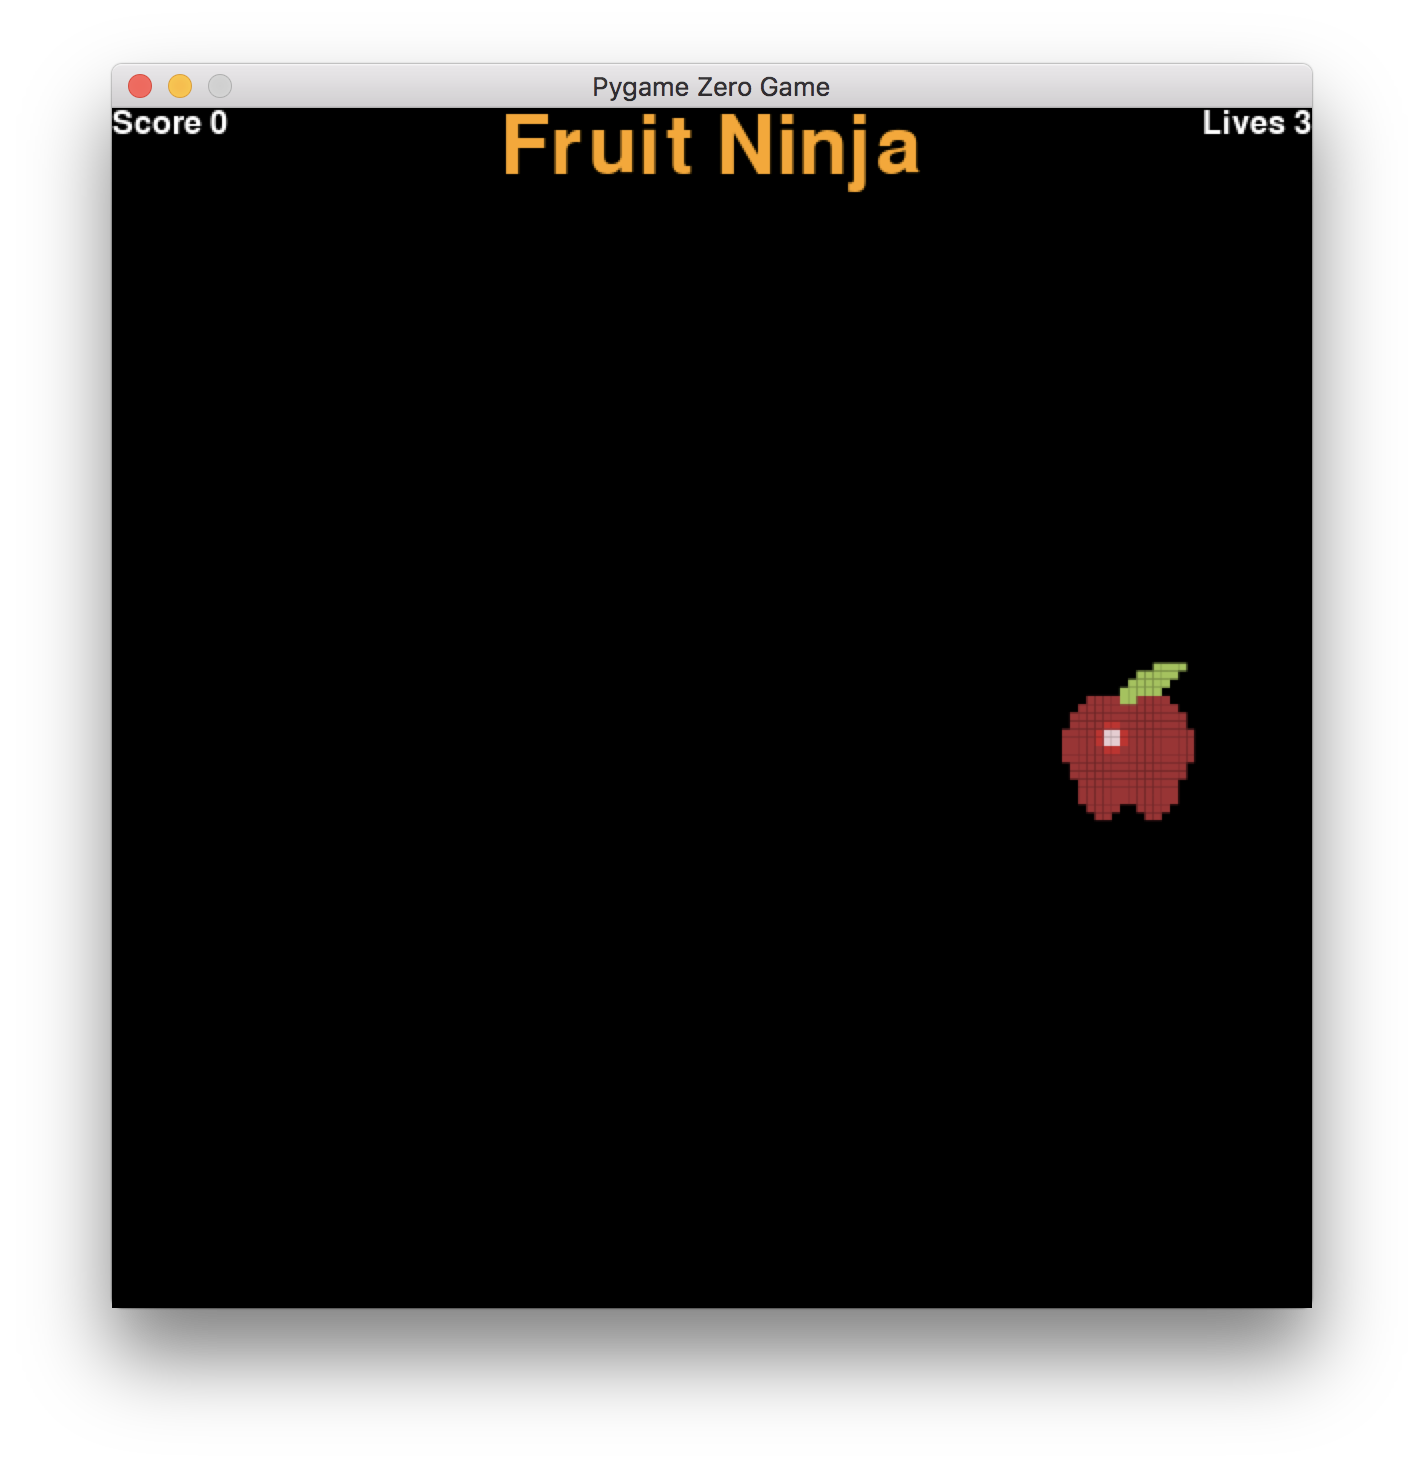
\includegraphics[width=.9\textwidth,clip,trim=0 600 0 0]{fruit_ninja_score}
\end{minipage}

The code to produce the game title and score is as follows:
\codeonly{listing options={firstline=13,lastline=16,numbers=none}}{13}{16}{\MUcode}{fruit_niinja_score.py}

\end{itemize}

\subsection{Multiple lives}

\TODO{Now you need to write similar code for multiple lives. You start with three lives and every time you miss a target you lose a life. When you have no lives left the game is over.}

\section{Moving targets}

Rather than placing the fruit in a random position we could make the game much more interesting by having moving fruit.  I think that the nicest effect is to `throw' fruit up from below the screen and have them fall back down due to gravity. This sounds complicated but it actually easy to do.

\TODO{Click on new file icon, \BUTTON{new}, and copy the code from \code{fruit_ninja_sounds} into this new file. Save, using icon \BUTTON{save}, as file \code{fruit_ninja_physics.py}. Finally, update the code as follows.}

\begin{center}
\begin{tikzpicture}
\node (P) {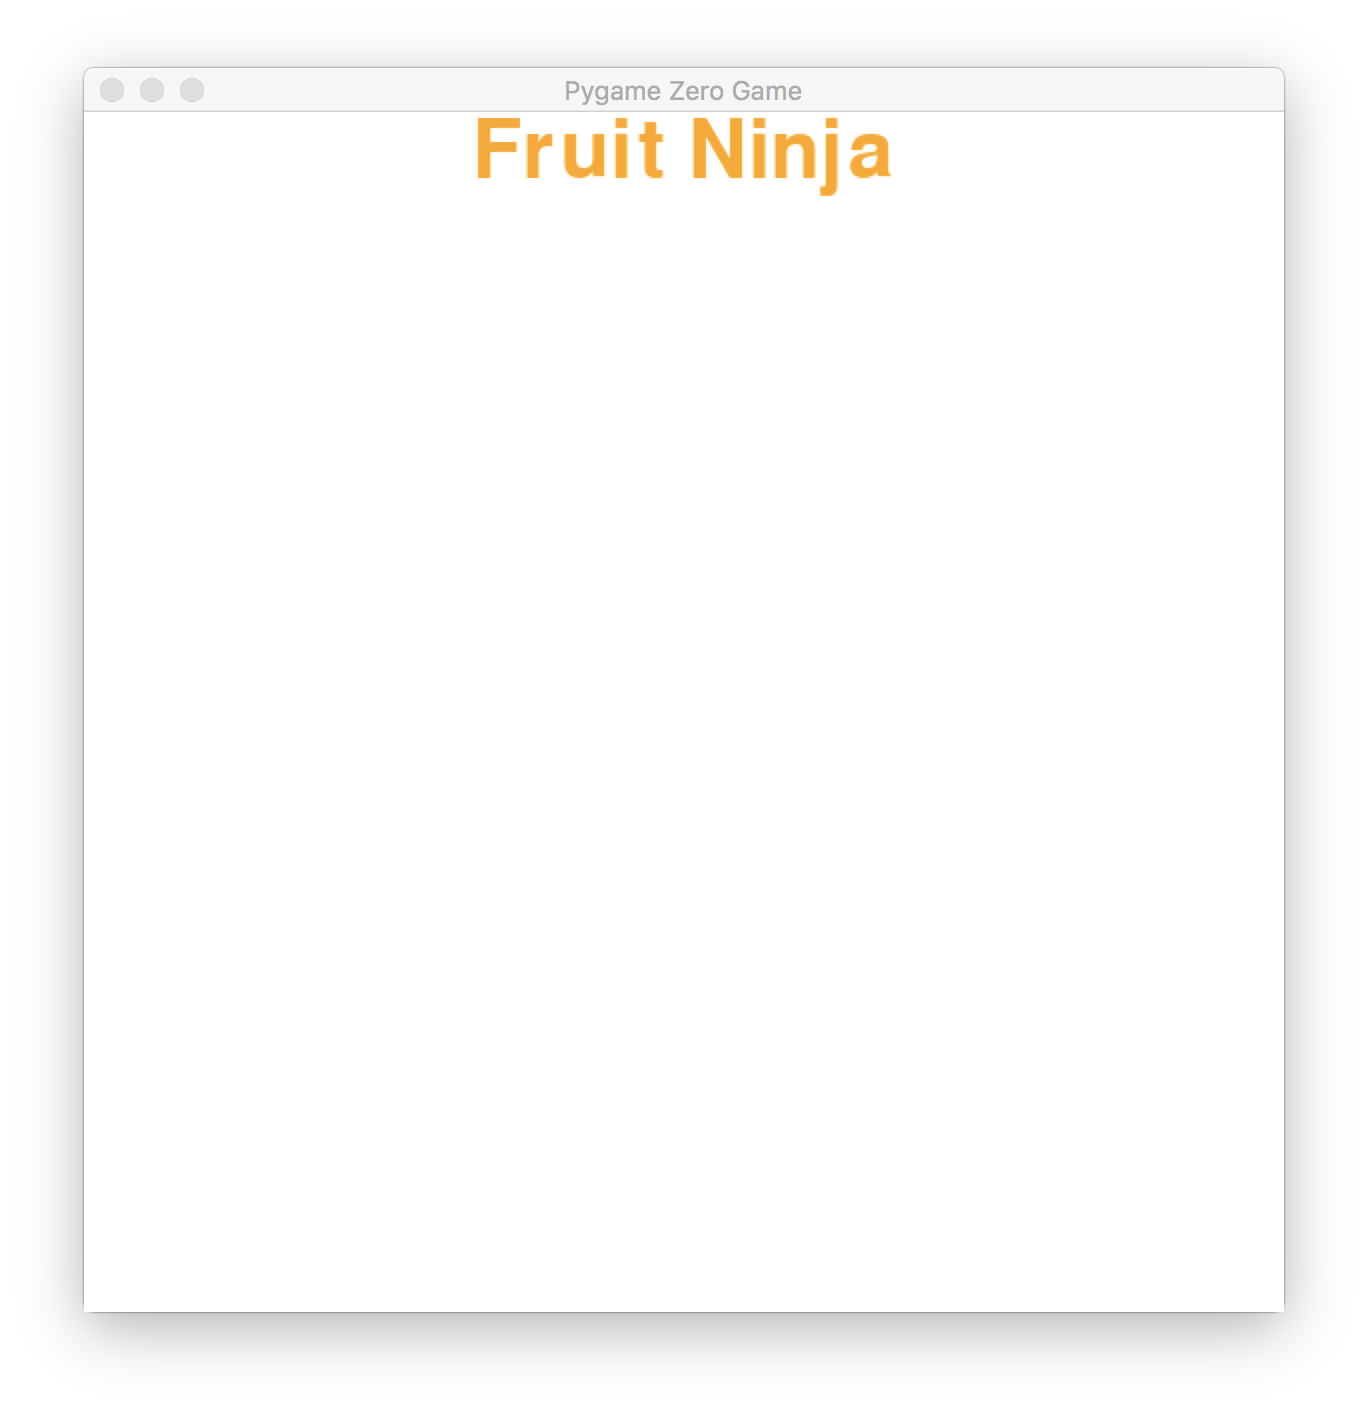
\includegraphics[width=9cm]{fruit_ninja_path}};
\draw[dashed] 
	($(P.south)+(-3,1)$) to[out=85,in=200] ++ (3,7) node {
\includegraphics[width=1cm]{apple}};
\draw[dashed] 
	($(P.south)+(3.5,1)$) to[bend right] ++ (-3,4) node {
\includegraphics[width=1cm]{apple}};
\node[draw,fill=yellow!10, drop shadow] at ($(P.south)+(0,0)$) {All fruit start below the screen};
\node[draw,fill=yellow!10, drop shadow, text width=5cm] at ($(P.south)+(0,2)$) {Fruit are thrown (nearly) upwards, and towards the centre };
\end{tikzpicture}
\end{center}

\begin{itemize}

\item[{\bf Step 0)}] {\bf Plan you code}.\\
The function \code{place_fruit} does a few things so lets be good programmers and plan what we are going to do.  

\TODO{Import the 2-dimensional vector from \code{pygame.math library} at the start of your program so that we can treat our horizontal ($x$) and vertical ($y$) movement together.}

\codeonly{listing options={firstline=3,lastline=3,numbers=none}}{3}{3}{\MUcode}{fruit_niinja_physics.py}

\TODO{Change the function \code{place_fruit} so it just contains the following comments. We will fill in the details or each in the following sections.}
\codeonly{listing options={firstline=1,lastline=8,numbers=none}}{1}{8}{code}{bits.py}

    \item[{\bf Step 1)}] {\bf Set the starting position}.\\
    We want the fruit to appear anywhere along the bottom edge of the screen --- so we set the $x$-coordinate to be random value in the range \code{20} to \code{WIDTH-20}.
    
    We want the fruit to appear from below the screen --- so we set the $y$ coordinate to be the screen height plus some margin.
     
\codeonly{listing options={firstline=22,lastline=25,numbers=none}}{22}{25}{\MUcode}{fruit_niinja_physics.py}

\item[{\bf Step 2)}] {\bf Set the starting velocity}.\\
We want the fruit to be thrown upward to a random height so \code{dy}, the velocity along the $y$-direction, is set to be a random value in range 10 to 20. These numbers were picked by trial and error, so the fruit would just go up to top of screen before falling back down.

\codeonly{listing options={firstline=27,lastline=28,numbers=none}}{27}{28}{\MUcode}{fruit_niinja_physics.py}

Note the minus sign. This is because $y$-direction points downwards.

If the $x$-direction component the velocity, \code{dx}, is zero then the fruit will just go directly up and then fall back down --- this is a bit boring. But if we set \code{dx} to a too large a value the fruit will fly past the side of the screen, and we won't have time to click on it. So we will change the sign of \code{dx} so that the fruit is thrown towards the centre.

\codeonly{listing options={firstline=29,lastline=31,numbers=none}}{29}{31}{\MUcode}{fruit_niinja_physics.py}

Finally, we now can set the velocity

\codeonly{listing options={firstline=32,lastline=32,numbers=none}}{32}{32}{\MUcode}{fruit_niinja_physics.py}

\item[{\bf Step 3)}] {\bf Set the acceleration}.\\

On Earth acceleration due to gravity is 9.81 metres per second squared, but in our game time does not run at the same rate so we can use a smaller value

\codeonly{listing options={firstline=34,lastline=35,numbers=none}}{34}{35}{\MUcode}{fruit_niinja_physics.py}


\item[{\bf Step 4)}] {\bf Update velocity and position}.\\

So now, all we have done is set the starting state of the fruit. How does it move? 

Physics --- or a sub-area of physics, called projectile movement --- comes to our aid. 

We have an object, an apple, that has position and velocity and is subjected to a fix acceleration\footnote{Remember, unlike in everyday speech, `acceleration' does not just mean we go faster. It means that our velocity changes, i.e. speed increases or decreases or/and direction changes.} (gravity) how does it move. We have two equations
\begin{align*}
	\text{velocity} \  =& \  \text{rate of change of position}\\
	\text{acceleration}  \  =& \   \text{rate of change of velocity}
\end{align*}

What is the `rate of change' of something? It is the change ($\text{new} - \text{old}$) divided by the length of time over which the change occurred. So we have 

\[
	(\text{velocity}) \ =  \ (\text{rate of change of position}) \ = 
	\ \frac{(\text{new position}) - (\text{old position})}{(\text{time duration})}
\]

Rearranging this we get
\[
(\text{new position})	= (\text{old position}) + (\text{time duration}) \times (\text{velocity})
\]
In our game world we will let (\text{time duration}) to be equal to one so the above equation to update position can be written as 
\codeonly{listing options={firstline=14,lastline=14,numbers=none}}{14}{14}{code}{bits.py}

We do this type of updating so often that python has an alternative, more compact, style
\codeonly{listing options={firstline=15,lastline=15,numbers=none}}{15}{15}{code}{bits.py}

Using the same logic we can go from equation
\[
\text{acceleration}  \  = \   \text{rate of change of velocity}
\] to python code
\codeonly{listing options={firstline=12,lastline=12,numbers=none}}{12}{12}{code}{bits.py}


We now want to run the two lines to update velocity and position over and over and over and over and \ldots.
We do this by defining the function \code{update} when is a special function that runs 60 times a second.

\TODO{Insert the following function.}

\codeonly{listing options={firstline=39,lastline=46,numbers=none}}{39}{46}{\MUcode}{fruit_niinja_physics.py}

Note:

\begin{itemize}
\item
We always update velocity before we update position. This will give us more accurate behaviour to help correct the fact that we only update 60 times a second but in reality Physcis is update continuously.
\item
When the fruit falls below the screen again, we `throw' a new fruit.
\end{itemize}
\end{itemize}

Update: 
You can also get a rotating effect by changing the property \code{angle} of you fruit.

\section{Multiple targets (and not all fruit!)}

We have one final improvement to make to our game. Rather than always throwing an apple we could throw different fruit. Or even better sometimes throw non-fruit items which we are NOT to click on.  

I won't write the steps to do this here --- instead we will cover this in the dojo --- however we need some images.

\vspace{3pt}
\begin{minipage}{.7\textwidth}
For game art, I like the site \href{https://www.gameartguppy.com/product-category/game-art-character-sprites/}{www.gameartguppy.com} which was developed by Vicki Wenderlich to ``give game devs who can't afford custom art (yet) an easy way to find and use free and inexpensive art.''
\end{minipage}
\begin{minipage}{.29\textwidth}\centering
\begin{tikzpicture}
\node (L) {
\includegraphics[width=.9\textwidth]{gameartguppy}};
\node at (L.south) {
\includegraphics[width=1cm]{Vicki_Wenderlich}};

\end{tikzpicture}
\end{minipage}

I have put in some of the food collection of images that I downloaded from 
\href{https://www.gameartguppy.com/product-category/game-art-character-sprites/}{www.gameartguppy.com} into \code{coderdojo-tramore/resources} folder.

\end{document}
%: END















SOFTWARE

https://docs.krita.org/en/index.html#

http://programarcadegames.com/python_examples/show_file.php?file=platform_jumper.py

https://www.instructables.com/id/Create-Your-First-Racing-Game/

https://github.com/CoderDojoLu

 https://www.zapsplat.com/page/2/?s=target&post_type=music&sound-effect-category-id

\section*{Introduction}

Today we are going to use our hard working turtles to build some holiday e-cards. You can build anything you wish, for example, the following are based on examples I found online

\begin{figure}[H]
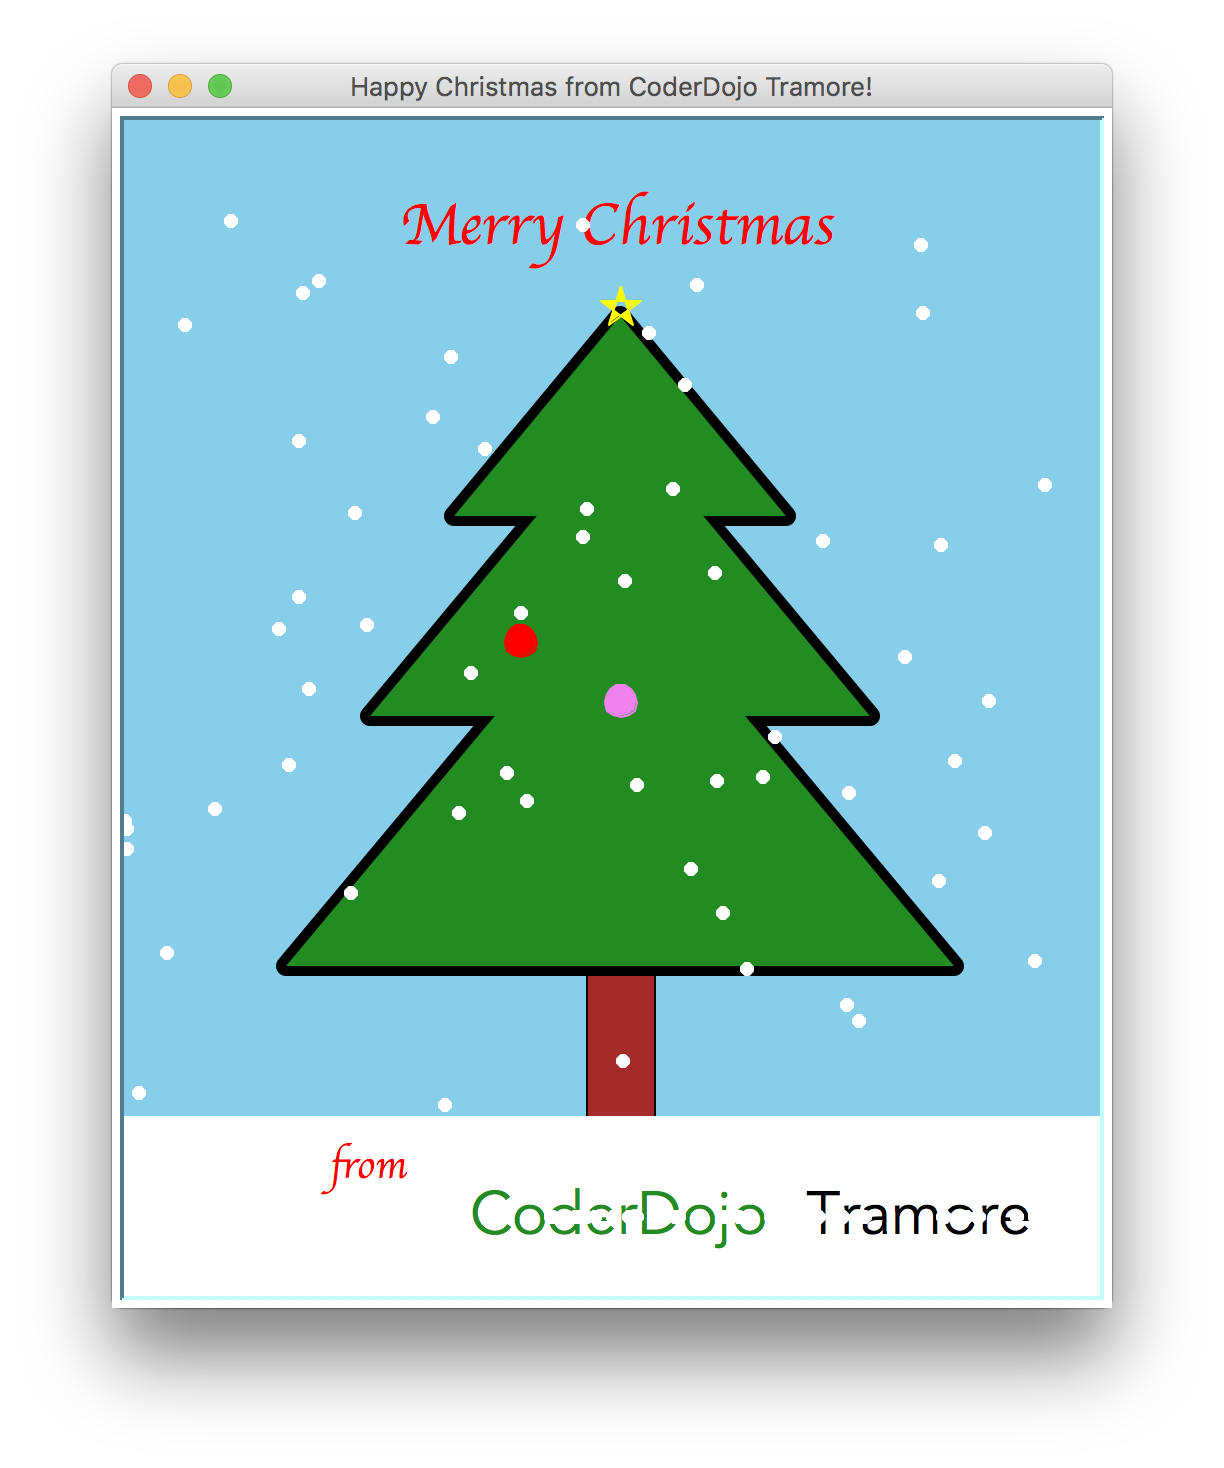
\includegraphics[height=5cm]{tree_final}
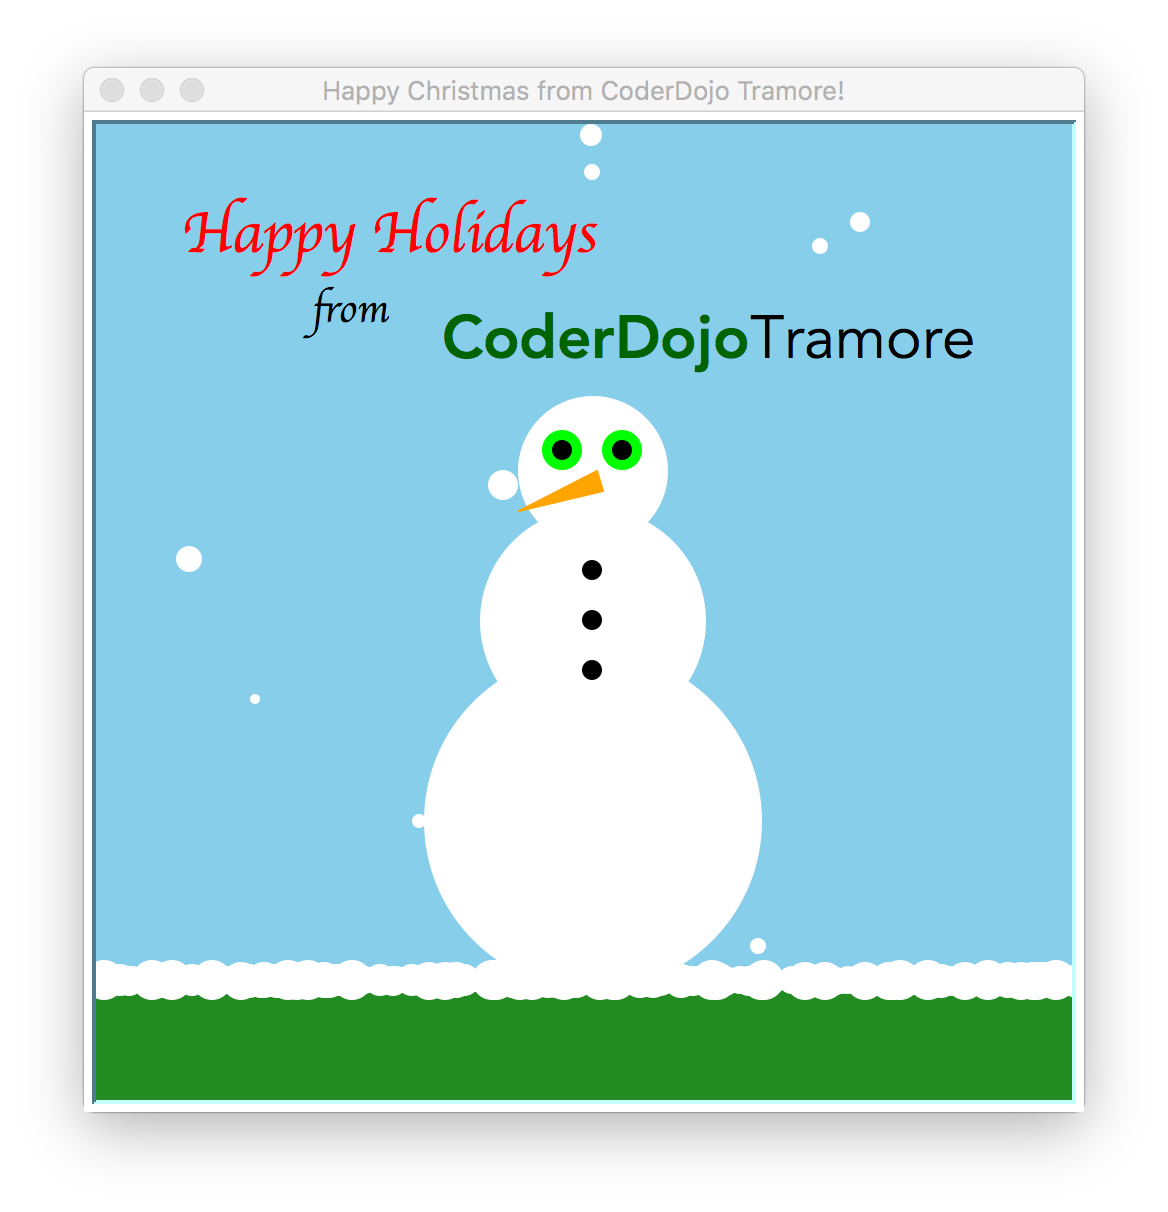
\includegraphics[height=5cm]{snowman_final}
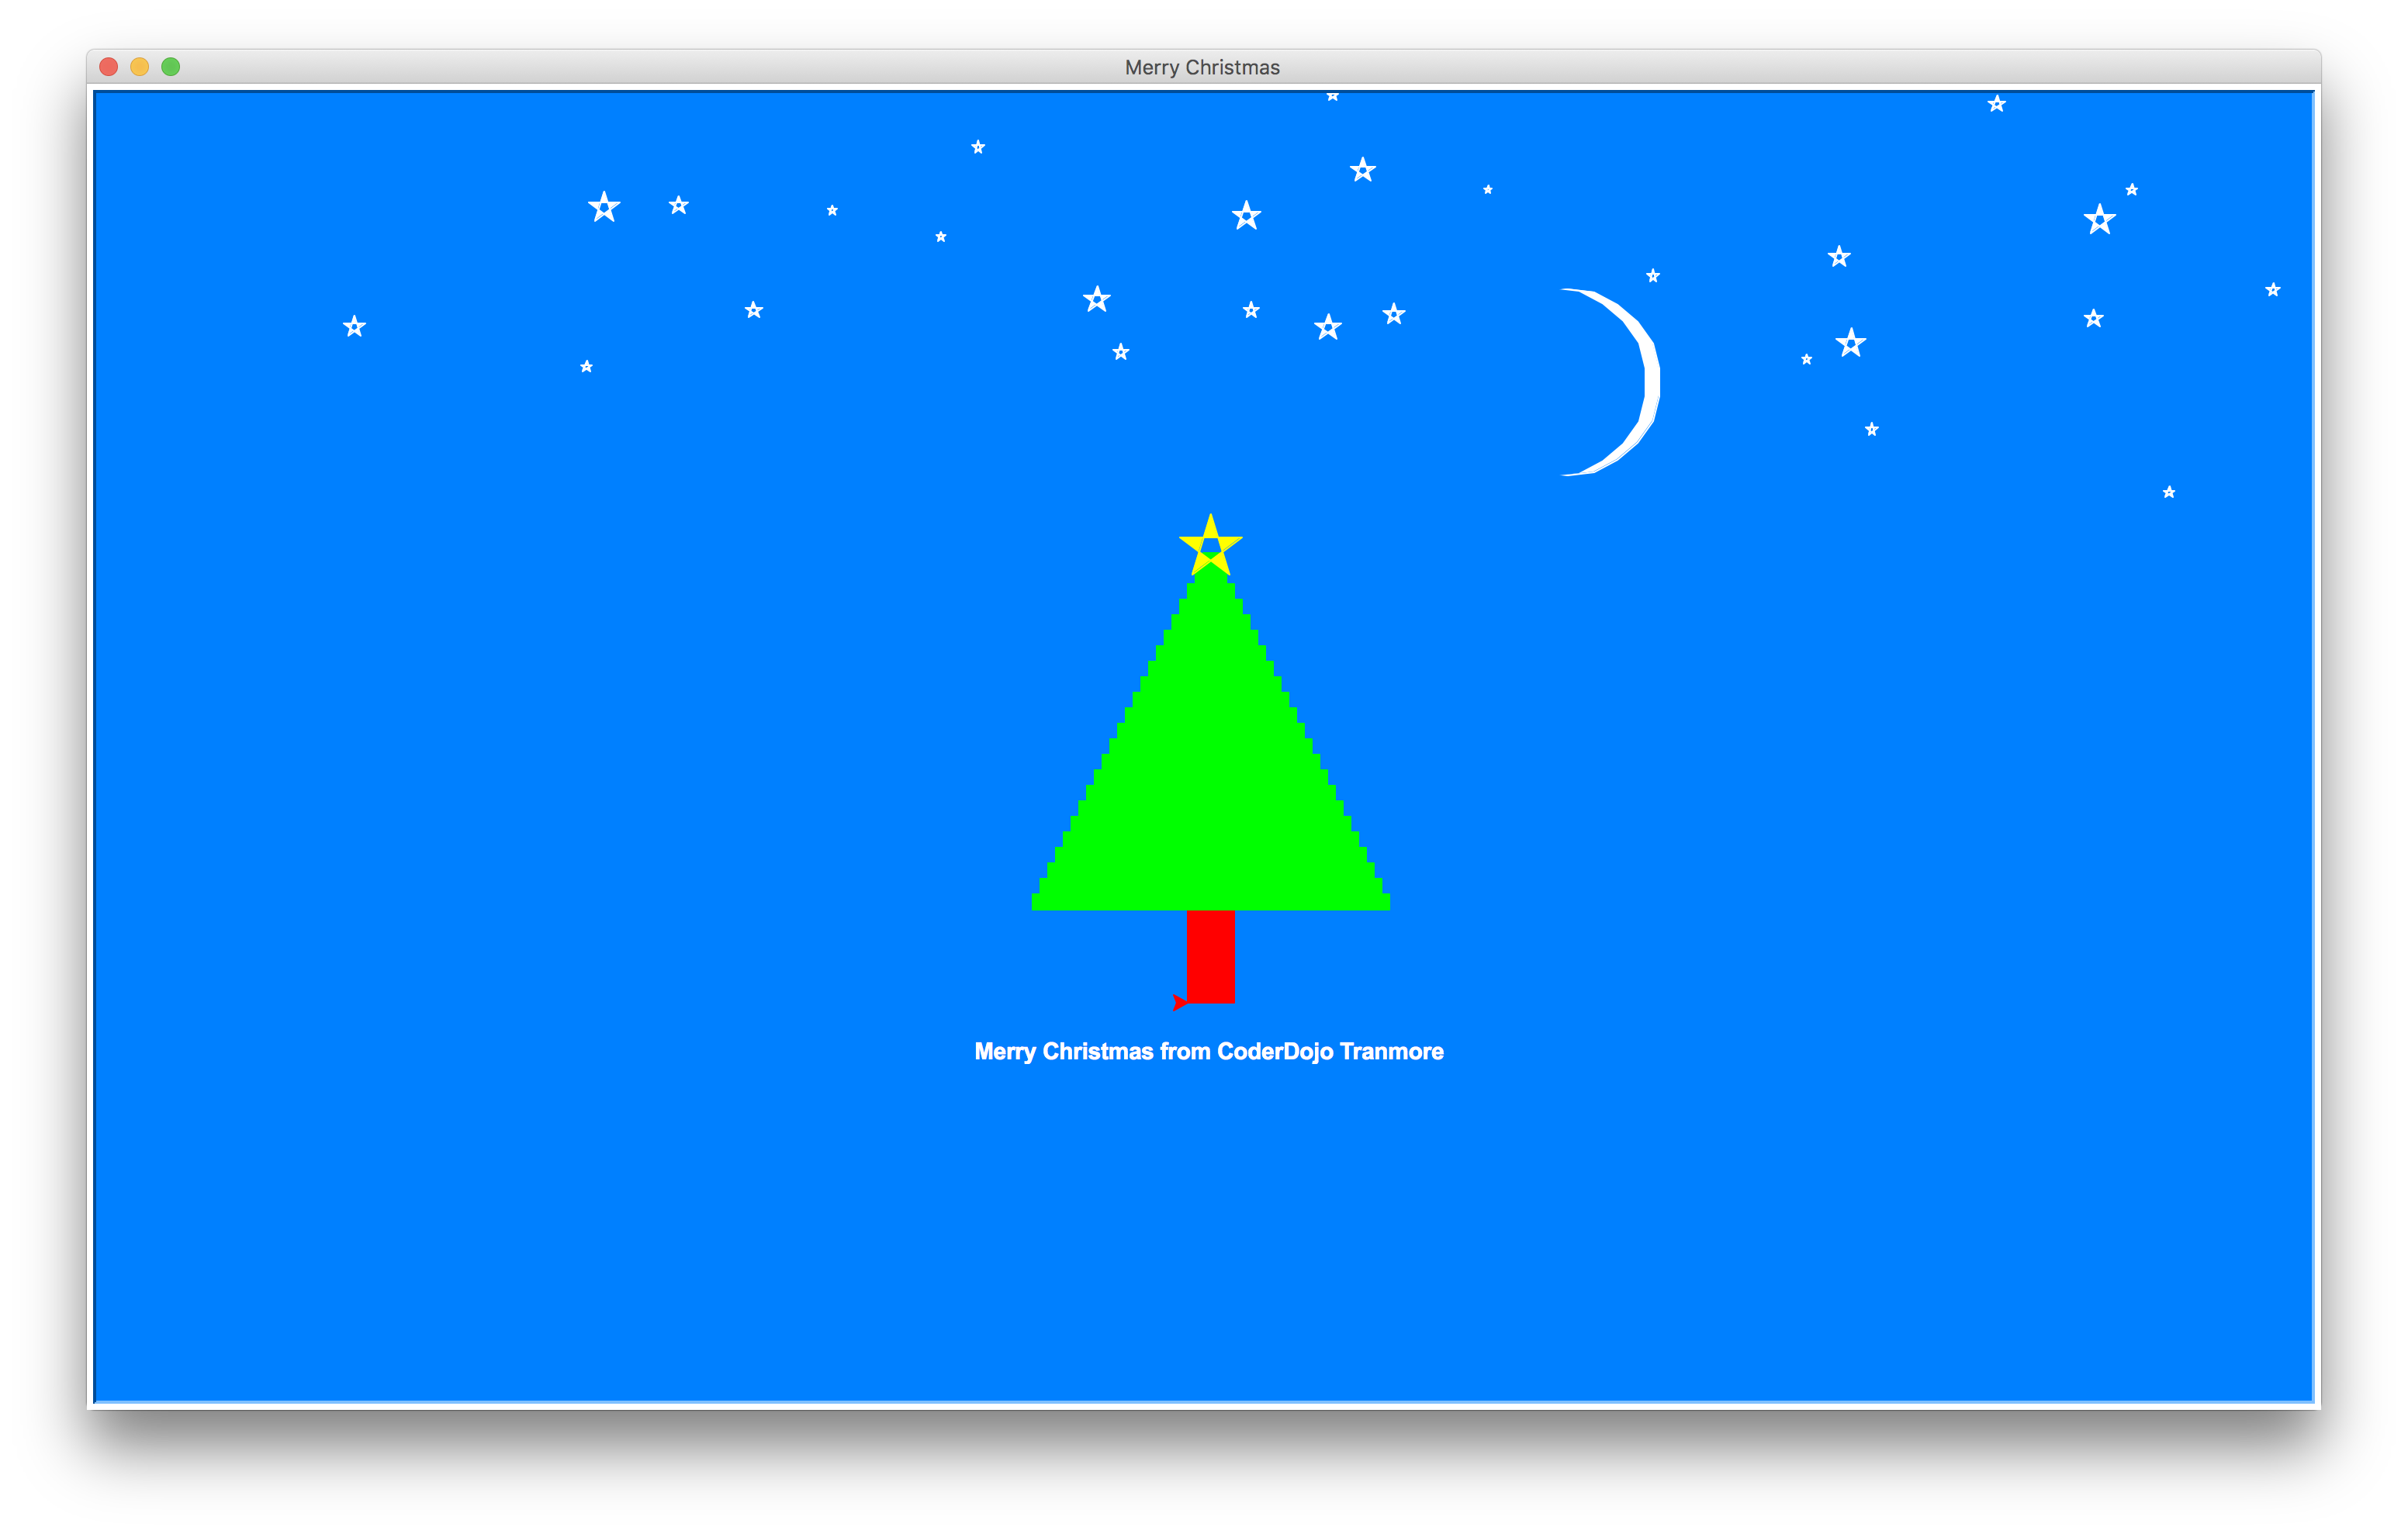
\includegraphics[height=5cm]{sky_final}\\
\mbox{}\hfill\raisebox{0pt}[0pt][0pt]{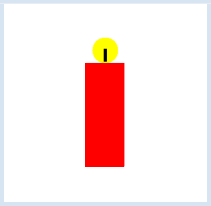
\includegraphics[height=2cm]{candle}}
\end{figure}

\vspace{-12pt}
I will go over the steps the build the first e-card and the rest is up to you!

First to help things along, we are going to change the way we use turtle graphics. Instead of starting our programmes with the code

\codeonly{}{1}{6}{code}{bits.py}  

we are going to use a small library called \code{my_library} as follows

\codeonly{}{8}{10}{code}{bits.py}  

This library has functions to:

\begin{dingautolist}{192} 
\contentsitem{ball}{Draw a ball}\\
\code{draw_ball(x, y, radius, color, fill_color)}
\contentsitem{rectangle}{Draw a rectangle}\\
\code{draw_rectangle(x, y, width, height, color, fill_color)}
\contentsitem{triangle}{Draw a triangle}\\
\code{draw_triangle(x, y, base, height, color, fill_color)}
\contentsitem{star}{Draw a star}\\
\code{draw_star(x, y, size, color, fill_color)}

\end{dingautolist}


\clearpage

\section{Before we start --- let's test our library}

\TODO{Create file called \code{test_my_library.py} and insert the following code.}

\codeonly{title={\code{test_my_library.py}}}{1}{120}{code}{test_my_library.py}  
\mbox{}\hfill\raisebox{0.5cm}[0pt][0pt]{%
	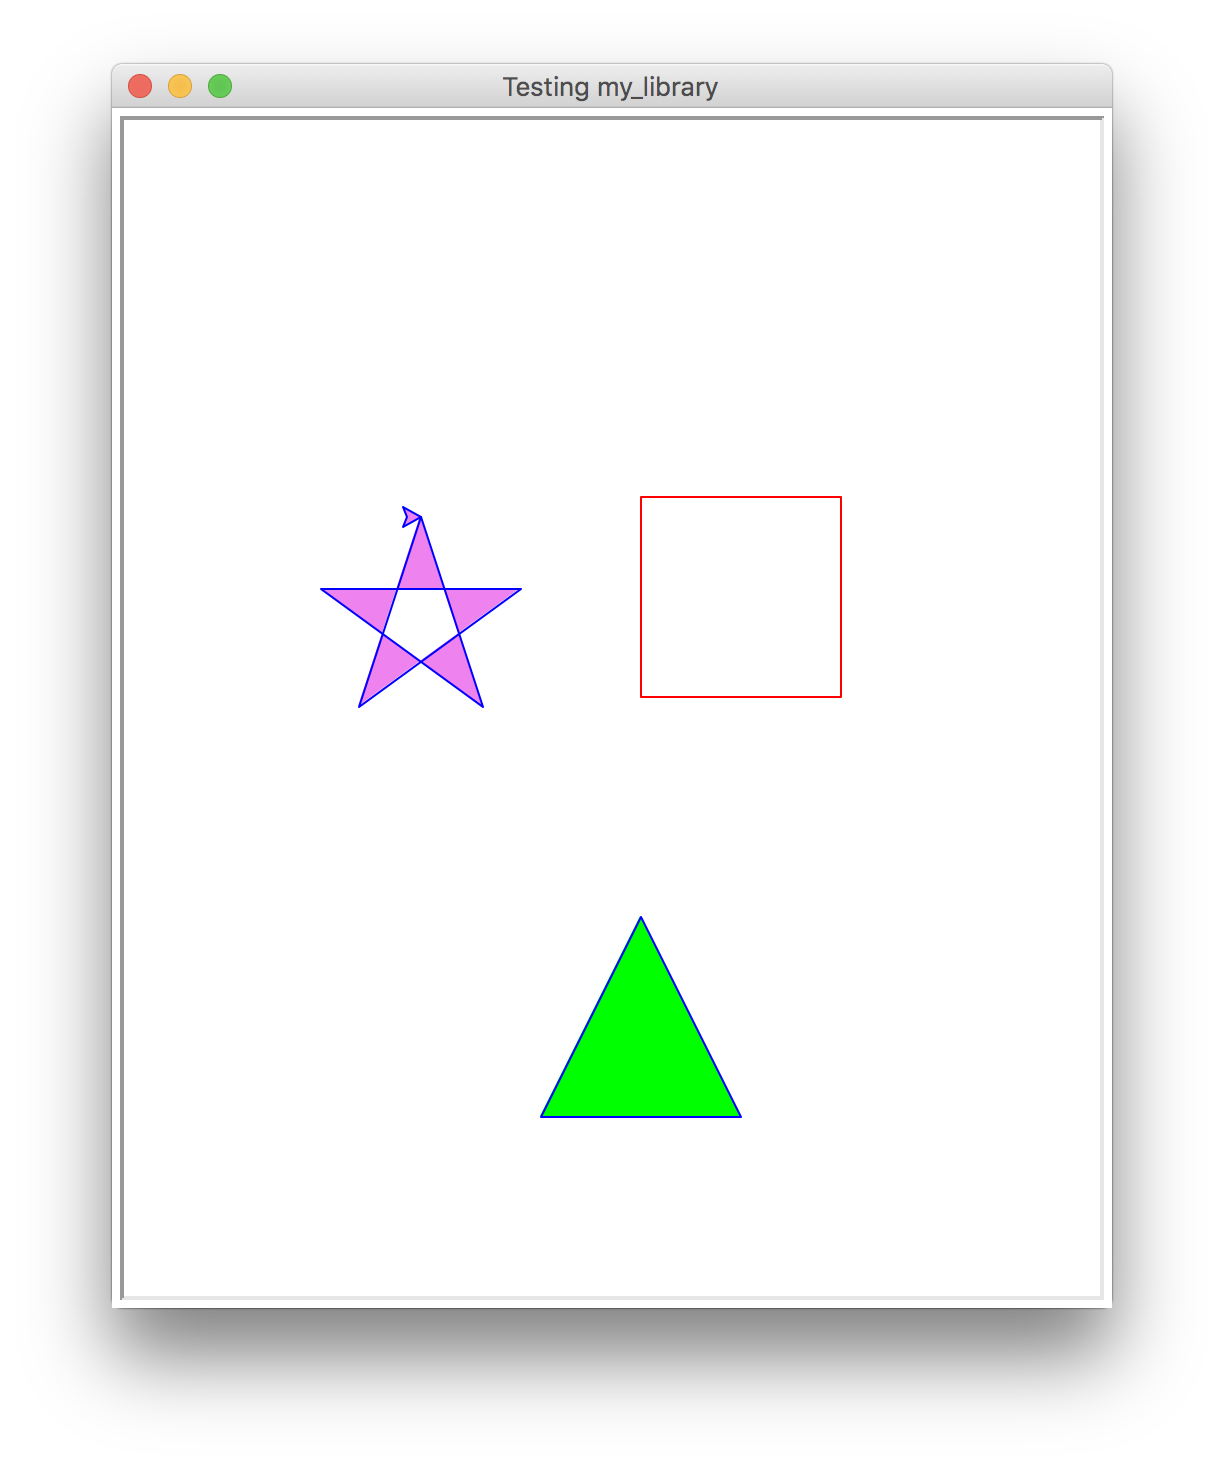
\includegraphics[width=5cm]{test_my_library}
}\hspace*{-1.5cm}


\section{Our First Card --- A Tree with Decorations}

Let's start by creating the tree with decorations example I showed you earlier. We will need to

\begin{minipage}{.6\textwidth}
\begin{dingautolist}{192} 
\contentsitem{screen}{Setup the screen (window)}
\contentsitem{tree}{Draw the tree}\\
I used three triangles and one rectangle for the trunk.
\contentsitem{ground}{Draw the sky and ground}\\
I changed the background colour and use a rectangle for the ground.
\contentsitem{decorations}{Draw the decorations}\\ I used balls, but only two so it is a bit sad. 
\contentsitem{message}{Write our message}
\contentsitem{snow}{Generate moving snow}\\ I used a new turtle for each snowflake.
\end{dingautolist}
\end{minipage}
\begin{minipage}{.35\textwidth}\centering
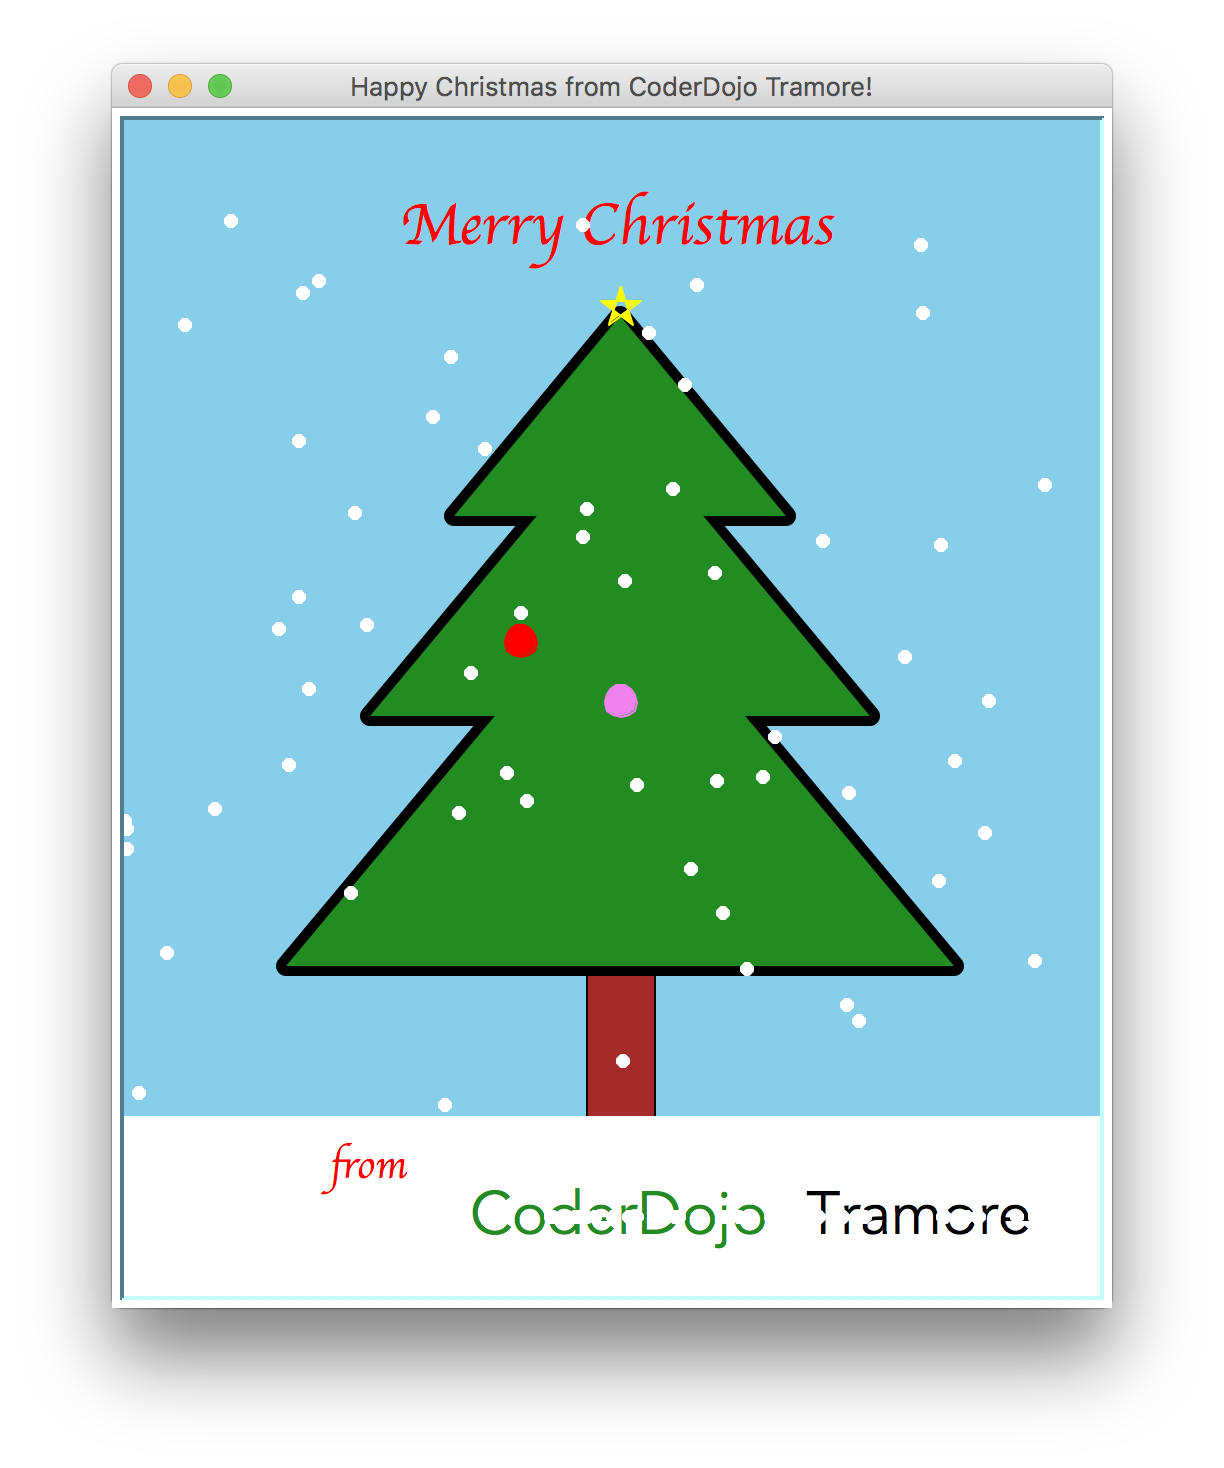
\includegraphics[height=8cm]{tree_final}
\end{minipage}

\vfill

\centerline{\tikz\node[label={[label distance=-12pt]90:\tikz\node[draw,fill=red!20]{\bfseries Note};},inner sep=12pt,draw,fill=red!5,rounded corners=12,drop shadow,text width=.9\textwidth] 
{I decided to make all distances relative to the width and height of the card. This make the drawing commands a little more complicated but I think you all can handle it. Please ask me to explain anything you don't understand. {\bf Remember, never just type code you don't understand --- I could be just stealing your credit card number!}
};}

\vfill\mbox{}

\clearpage
\subsection{Setup the screen}\label{sec:screen}

\TODO{Create file called \code{tree_with_decorations.py} and insert the following code.}

\codeonly{title={\code{tree_with_decorations}}}{1}{120}{code}{tree_with_decorations_1.py}  
\mbox{}\hfill\raisebox{8cm}[0pt][0pt]{%
	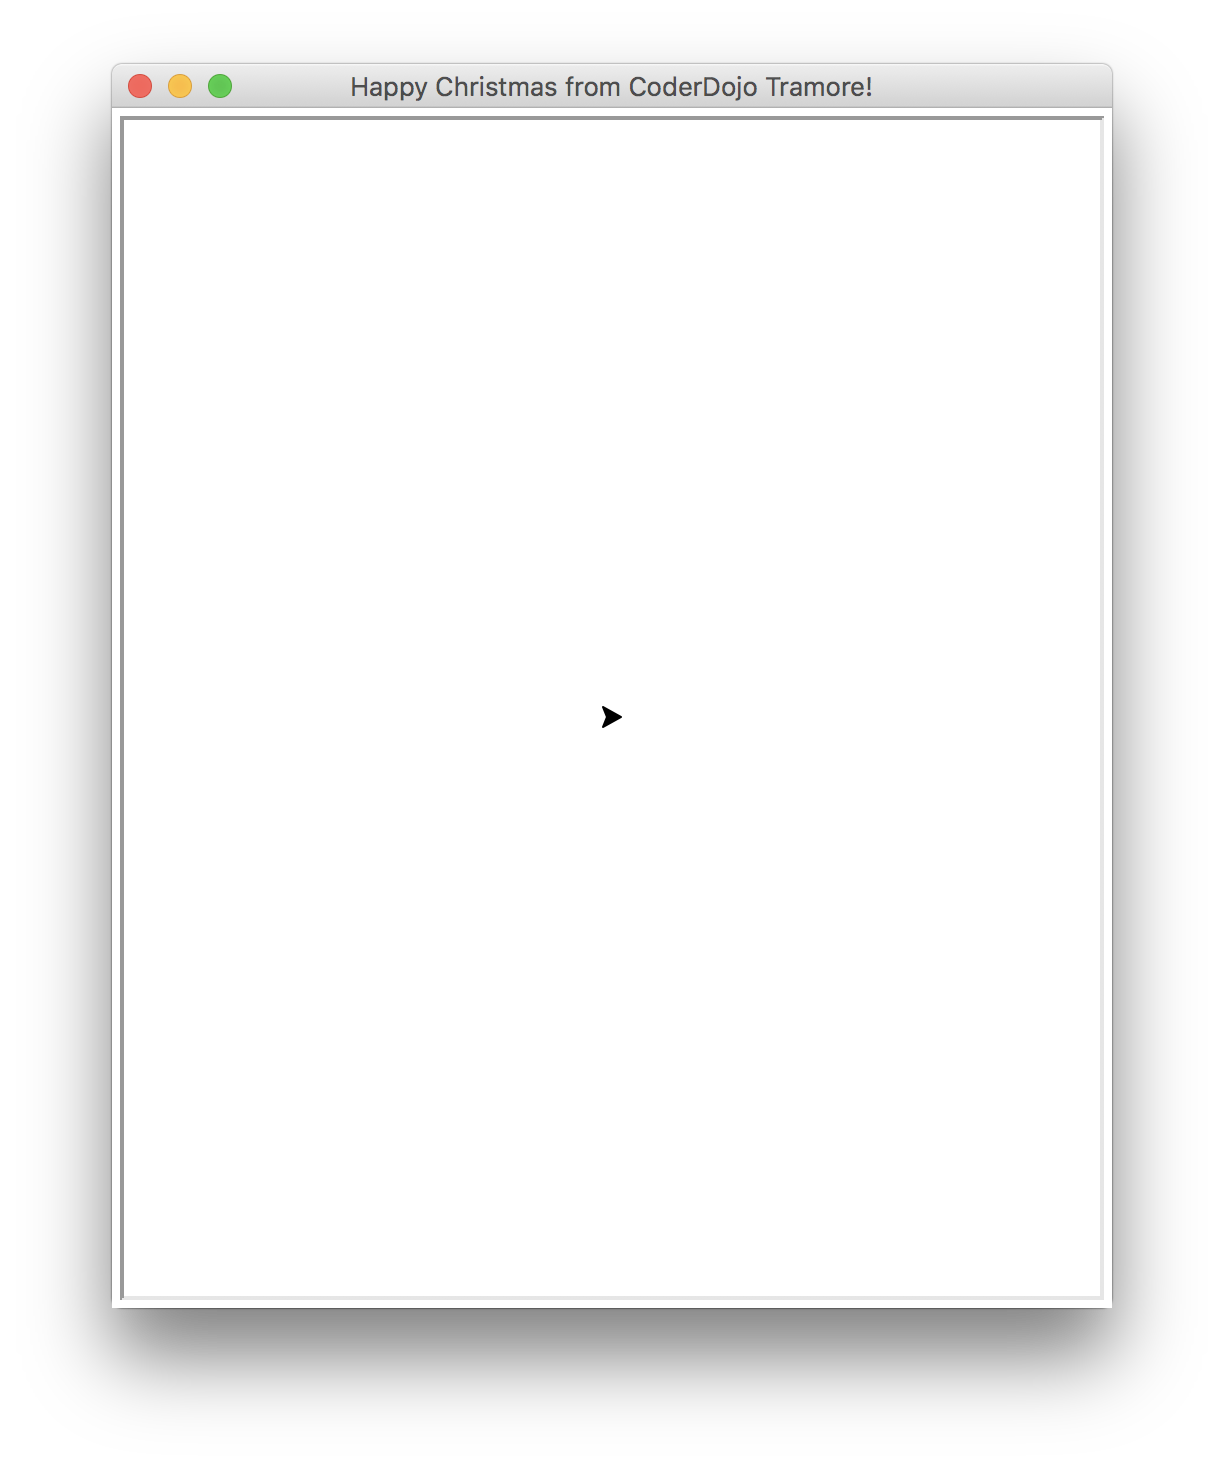
\includegraphics[width=5cm]{tree_with_decorations_1}
}\hspace*{-1.5cm}

Note:
\begin{itemize}
\item This is a relatively complex scene so all of the comments in the above file are placeholders to help use keep our code organised --- always a good idea. All of the drawing will be in section \code{### my drawings ###} and any data and functions that I need to create my drawings will be in \code{### my data ###} and \code{### my functions ###} respectively.
\end{itemize}

\subsection{Draw the tree}\label{sec:tree}

Drawing the tree trunk is easy --- it is just a rectangle.

\TODO{Insert the following line into \code{tree_with_decorations.py} {\bf at the appropriate section.}}

\codeonly{title={\code{tree_with_decorations}}}{17}{18}{code}{tree_with_decorations_2.py}  
\mbox{}\hfill\raisebox{0cm}[0pt][0pt]{%
	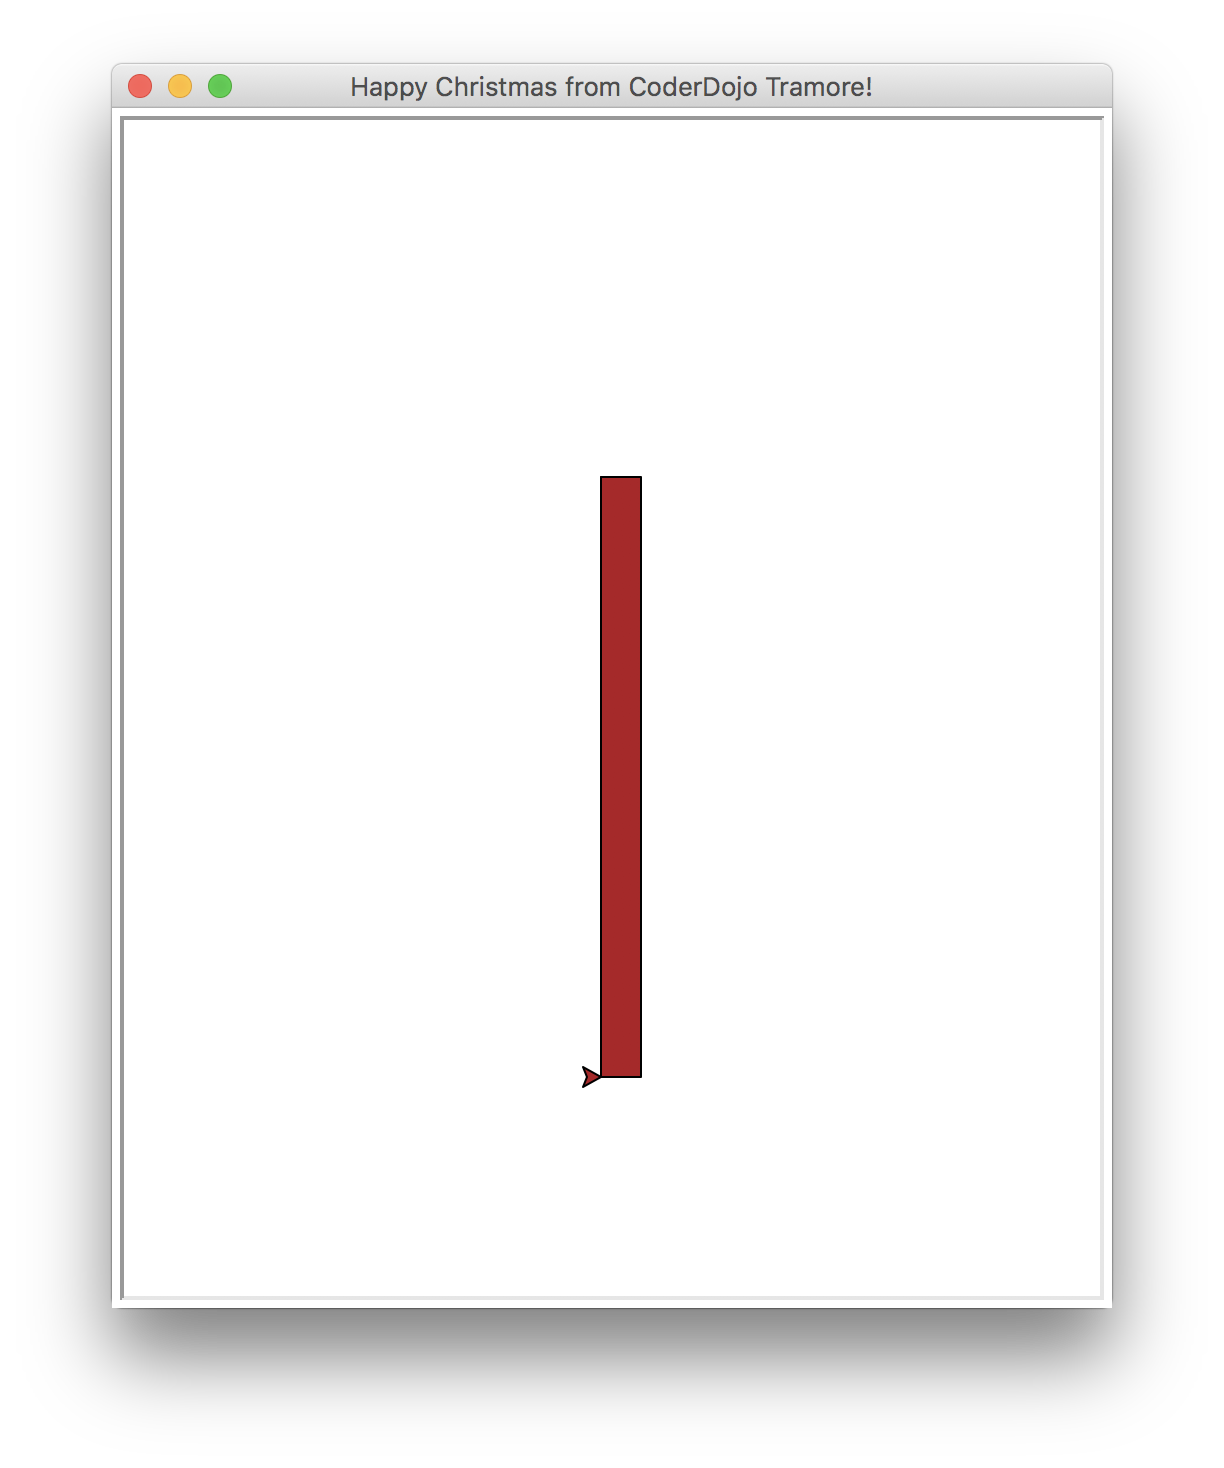
\includegraphics[width=1.5cm]{tree_with_decorations_2a}
}\hspace*{-1cm}

To get a nice looking tree I draw it twice. First drawing the outline using a thick pen in black, then a second time only drawing the inside. 

\TODO{Insert the following line into \code{tree_with_decorations.py} {\bf at the appropriate section.}}

\codeonly{title={\code{tree_with_decorations}}}{20}{27}{code}{tree_with_decorations_2.py}  
\mbox{}\hfill\raisebox{3.2cm}[0pt][0pt]{%
	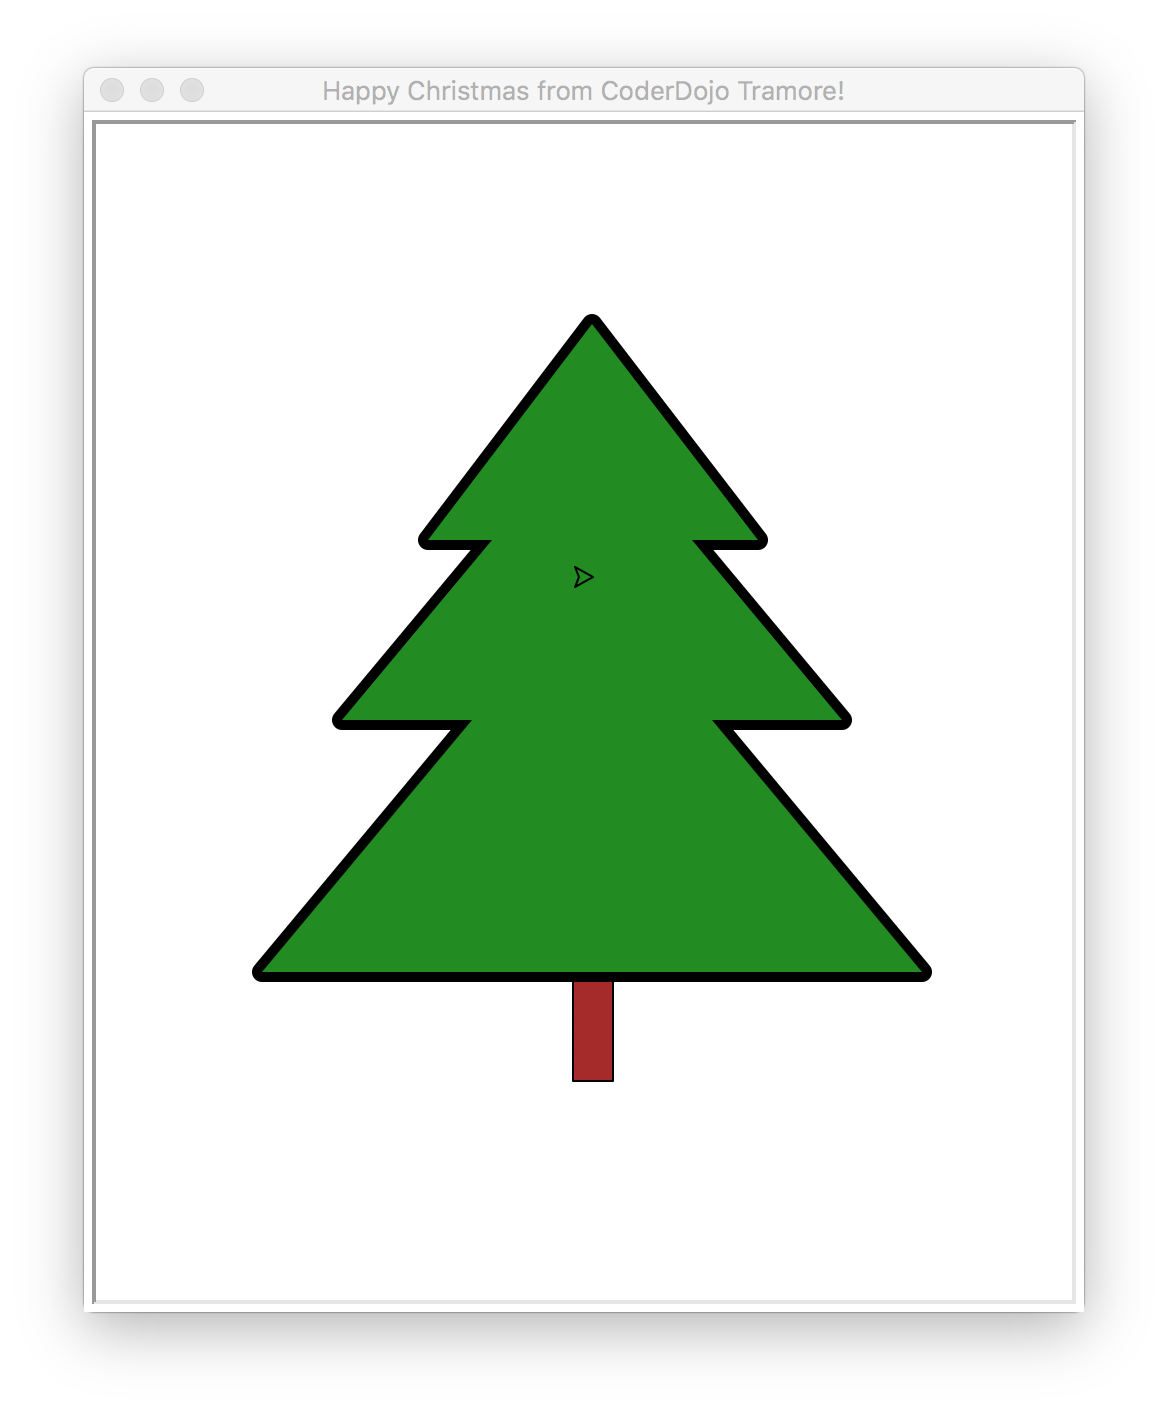
\includegraphics[width=3cm]{tree_with_decorations_2b}
}\hspace*{-1cm}

\subsection{Draw the sky and ground}\label{sec:ground}

\TODO{Insert the following line into \code{tree_with_decorations.py} {\bf at the appropriate section.}}

\codeonly{title={\code{tree_with_decorations}}}{13}{15}{code}{tree_with_decorations_2.py}  
\mbox{}\hfill\raisebox{0.5cm}[0pt][0pt]{%
	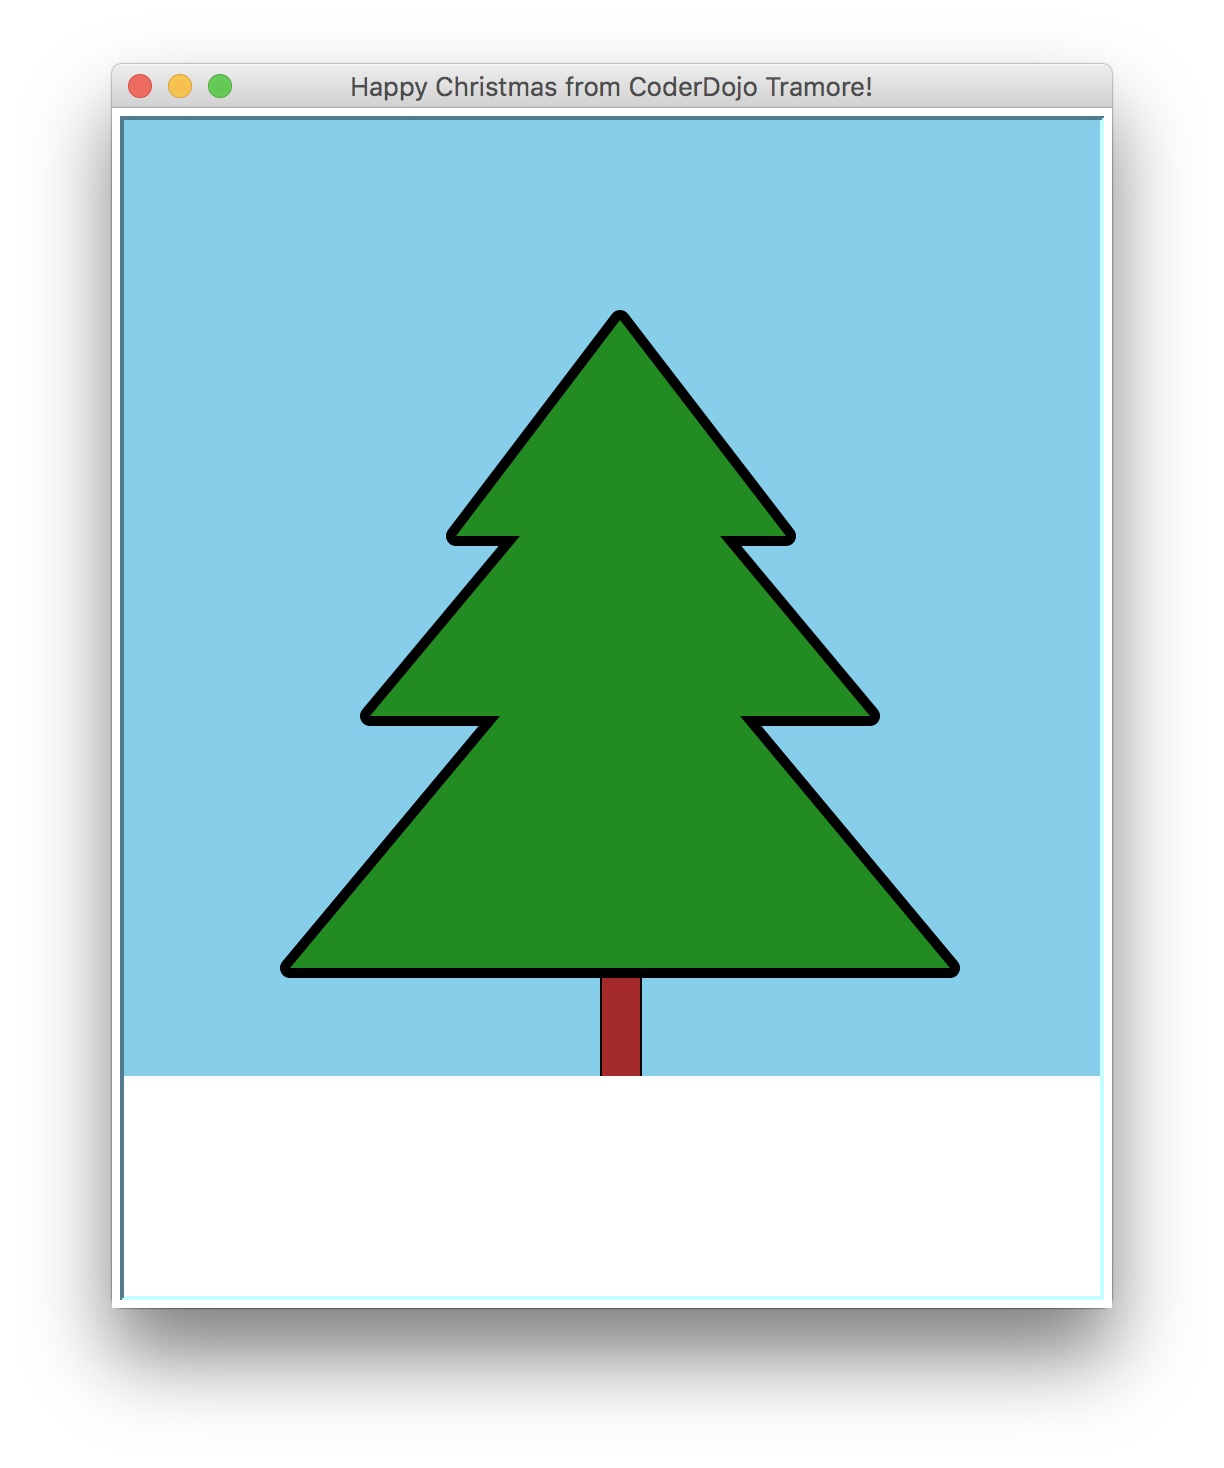
\includegraphics[width=2cm]{tree_with_decorations_2d}
}\hspace*{-1cm}

Notice the commented line. We will uncomment this later, it is easier to see if something goes wrong if we can see the turtle moving.

\TODO{
The ground is just a rectangle --- As a test of your understanding of the code so far, you will have to come up with the line to draw the ground yourself!}

\subsection{Draw the star}\label{sec:star}

\TODO{
You draw the star using \code{draw_star} comment  --- let's see if you can place that yourself!}

\clearpage

\subsection{Draw the decorations}\label{sec:decorations}

The decorations are a number of balls placed at various points on the tree.  We could pick random positions but it usually generates clumps of decorations and we want them to be more spread out\footnote{%
This is a common issues with generating random data --- it often has bigger clumps than we would like. The solution to this is to use \href{https://www.johndcook.com/blog/2009/03/16/quasi-random-sequences-in-art-and-integration}{quasi-random} which is distinct from \href{http://www.haifux.org/lectures/79/random.pdf}{pseudo-random}.} So we will manually set the position and colour of each ball. In the following code I have created two decorations --- you should try to add more yourself.

\TODO{Insert the following line into \code{tree_with_decorations.py} {\bf at the appropriate section.}}

\codeonly{title={\code{tree_with_decorations}}}{36}{40}{code}{tree_with_decorations_2.py}  
\mbox{}\hfill\raisebox{-0.5cm}[0pt][0pt]{%
	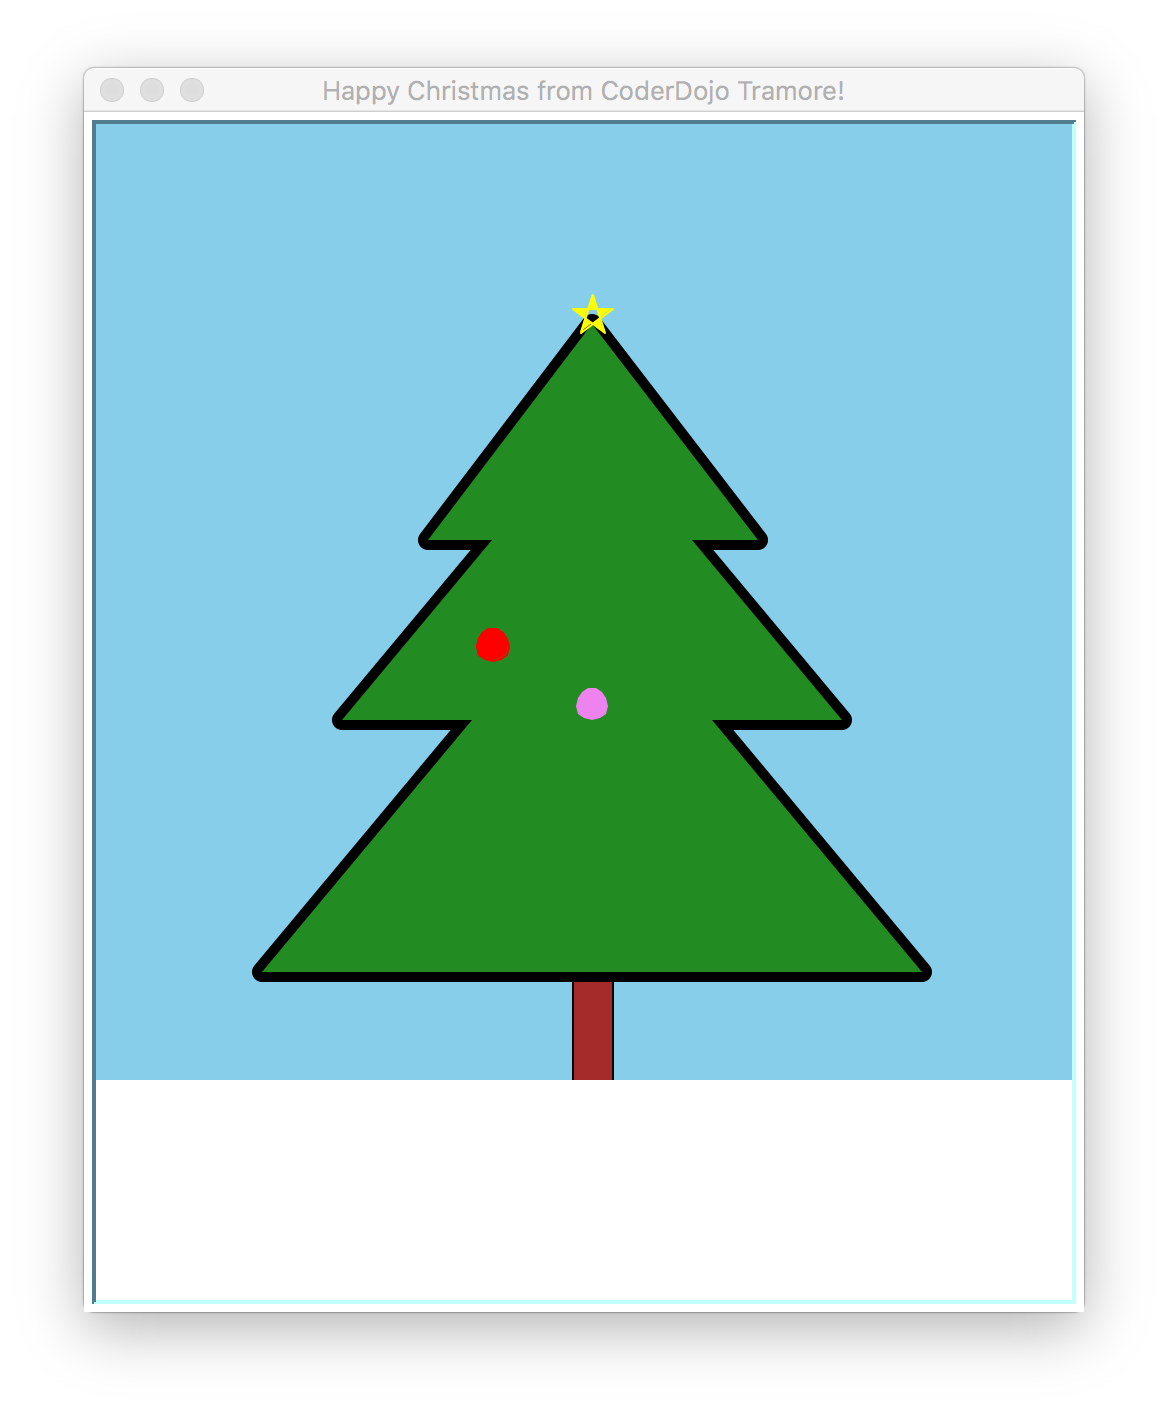
\includegraphics[width=4cm]{tree_with_decorations_2f}
}\hspace*{-1cm}

\TODO{Add more decorations!}

\subsection{Write our message(s)}\label{sec:message}

To write a message we:
\begin{itemize}
\item Move our hard working turtle, \code{bob}, to the desired position.
\item Set the colour we want for the message.
\item Pick the font family, size, and weight (bold, normal).
\item Tell \code{bob} what to write.
\end{itemize}

\TODO{Insert the following line into \code{tree_with_decorations.py} {\bf at the appropriate section.}}

\codeonly{title={\code{tree_with_decorations}}}{42}{46}{code}{tree_with_decorations_2.py}  
\mbox{}\hfill\raisebox{0.5cm}[0pt][0pt]{%
	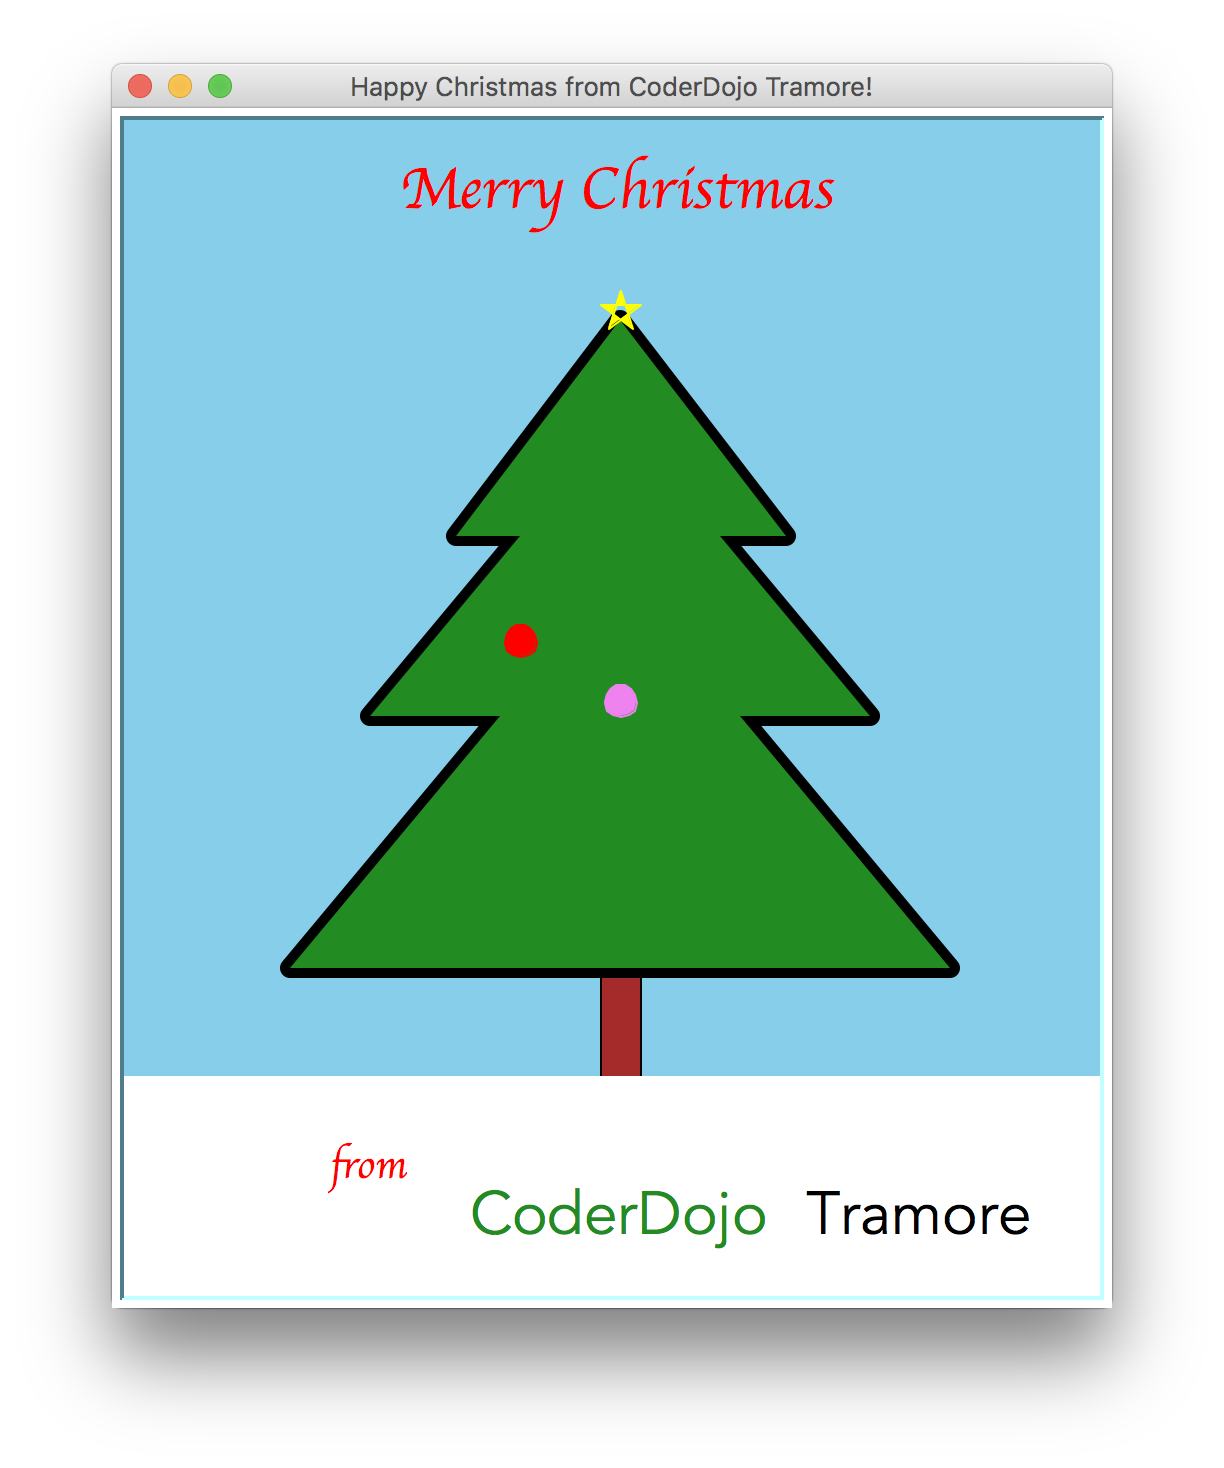
\includegraphics[width=3cm]{tree_with_decorations_2h}
}\hspace*{-1cm}

\TODO{Insert the code {\bf at the appropriate sections} needed to generate all of the text in the above figure.}


\clearpage

\subsection{Generate moving snow}\label{sec:snow}

OK, to get snowflakes falling, we are going to create A LOT OF TURTLES, each turtle will represent a snowflake. This might appear crazy, but it works if:

\begin{itemize}
\item
We change how the turtles appear by changing their shape to a  '\code{circle}', changing their colour to \code{white}, making them smaller.

\item 
We point the turtles downwards so that when they move forward they look like there are falling.

\item
We keep a list of all turtles so when they get to the bottom of the screen we \ldots\ `kill them off'.
\end{itemize}

\TODO{We need to keep a list of snowflakes so add the following code segments {\bf at the appropriate sections}.}

\codeonly{title={\code{tree_with_decorations}}}{7}{8}{code}{tree_with_decorations_3.py}  

Next we add our functions for creating and move the snowflakes

\codeonly{title={\code{tree_with_decorations}}}{10}{39}{code}{tree_with_decorations_3.py}  

Finally to see snow falling we need to insert the following code AFTER our `Merry Christmas' message code

\codeonly{title={\code{tree_with_decorations}}}{80}{82}{code}{tree_with_decorations_3.py}  

\TODO{Insert the above code after each message and at the end of your program insert the next bit of code (this parts will run forever.}

\codeonly{title={\code{tree_with_decorations}}}{108}{110}{code}{tree_with_decorations_3.py}  

\subsection{Exercises}

We are done \ldots\ but \ldots

\begin{itemize}
\item
What about having random sized snowflakes?
\item
What about adding a wind that causes the snowflakes to fall to the side?
\item
What about making the decorations sparkle?
\item
What about \ldots\ you get the idea!  
\end{itemize}
%: END
\end{document}




\vspace{6pt}
You could ask ``{\em Why?}'' as in ``{\em Why would we build our own menu system? Surely it is easier to use an existing GUI library?}''

\begin{minipage}{.5\textwidth}
The answer is: Yes, it would be easier, but we want to build our own because;

\begin{itemize}
\item We can.
\item We will use this to learn how GUI respond to events (mouse click, keyboard press/release, etc.).
\item We will be able to add our own special effects (more later) to our GUI.
\end{itemize}
\end{minipage}
\begin{minipage}{.5\textwidth}
\begin{figure}[H]
\centering
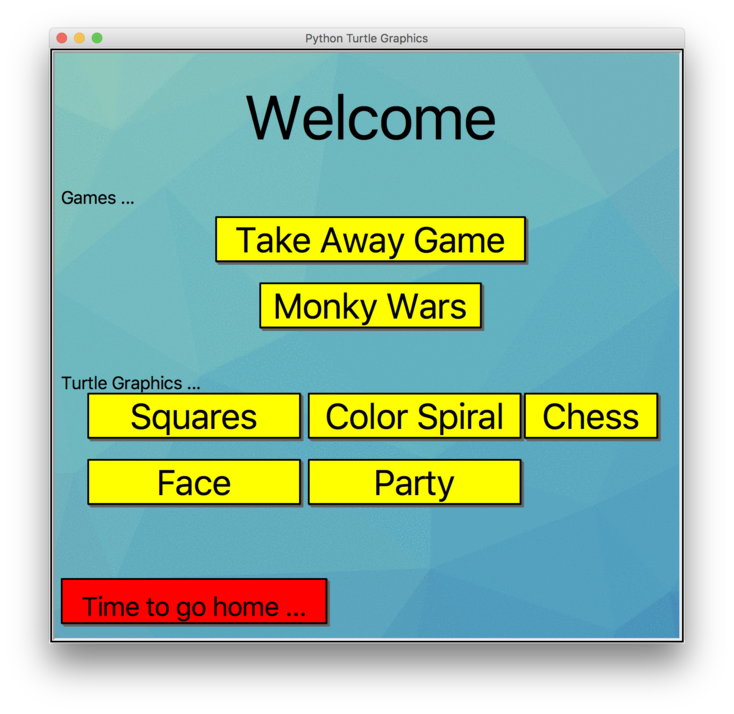
\includegraphics[width=6cm]{Menu_Complete}\\[-12pt]
\caption{Completed main menu.} 
\end{figure}
\end{minipage}

\vspace{6pt}
As usual we build this using a sequence of steps --- testing our code along the way.

\begin{dingautolist}{192} 
\contentsitem{screen}{Creating the Menu Screen}

We have done this many time before. All we need do is import the \code{turtle} module and create a \code{Screen} where we place our drawing, and a \code{Turtle} or two to do the actual drawing.  We do one thing that is new --- we insert a background image (must be in \code{gif} format).

\contentsitem{button}{Creating Buttons that Work}

Here we need to do some fancy coding --- both in drawing our buttons and figuring out how to respond to a button click.  

\contentsitem{take_away}{Building the Menu}

Finally, here you can design your menu screen anyway you want --- don't be stuck with my boring, everything is in a gird layout.

\contentsitem{button}{Updating our Earlier Programs so they Behave with Our Menu --- TODO}

We will need to modify some of our earlier programs (Graphical Take Away, Monkey Wars, etc) so they work better when we run them from our menu.  

This is a small task that we will leave until next week. Also we have yet to add the cool features!

\end{dingautolist}

\clearpage
\section{Creating the Menu Screen}\label{sec:screen}

\TODO{Create file called \code{Menu.py} and insert the following code.}

\codeonly{title={\code{Menu.py}}}{1}{120}{code}{Menu_Start.py}  
\mbox{}\hfill\raisebox{4cm}[0pt][0pt]{%
	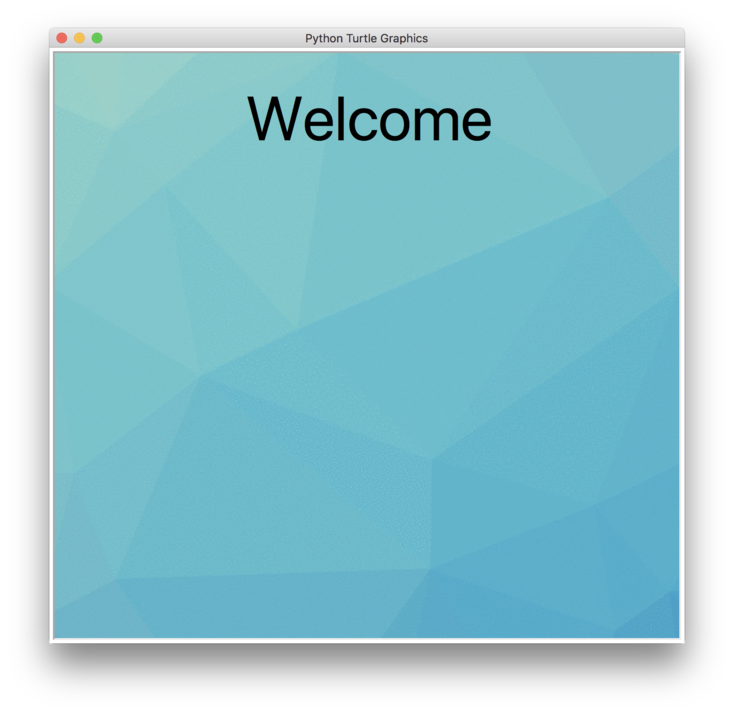
\includegraphics[width=9cm]{Menu_Start}
}\hspace*{-1.5cm}

Our code will get long so we need to keep things organised. Here the code is divided in to four sections --- import modules, create the empty screen and set background, define helper functions, and finally build the screen.

Currently this code just creates the window with the ``Welcome'' message. Next we will add buttons and mouse click events.
\clearpage

\section{Creating Buttons that Work}\label{sec:buttons}

\begin{figure}[H]
\centering\larger[2]\vspace{-18pt}
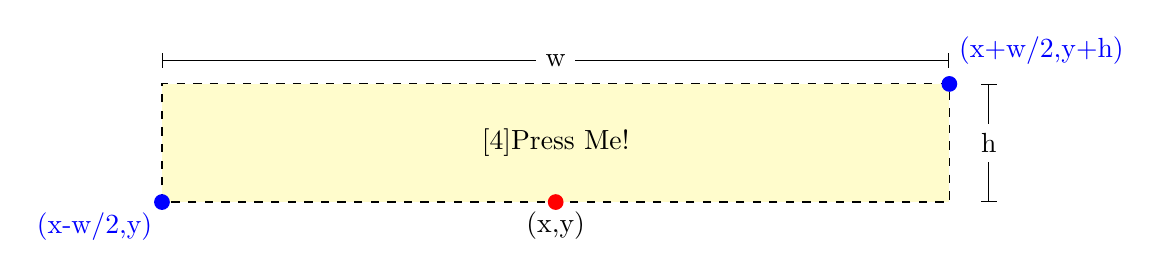
\begin{tikzpicture}
	\draw[dashed,fill=yellow!20] (-5,0) rectangle (5,1.5);
	\fill[red] (0,0) circle (.1) node[below,black] {(\code{x},\code{y})};
	
	\node[font={\larger[4]}]  at (0,0.75) {Press Me!};
	\draw[|-|] (5.5,0) -- node[fill=white] {\code{h}} ++(0,1.5); 
	\draw[|-|] (-5,1.8) -- node[fill=white] {\code{w}} ++(10,0); 
	\fill[blue] (-5,0) circle (.1) node[below,left,yshift=-9pt] {(\code{x}-\code{w/2},\code{y})};
	\fill[blue] (5,1.5) circle (.1) node[above,right,yshift=12pt] {(\code{x+w/2},\code{y+h})};
\end{tikzpicture}
\caption{Button position and dimensions.\label{fig:button}}
\end{figure}

\subsection{Developing a function to build a Button}

In order to create a button that we can click we need to decide on its:
\begin{itemize}
\item Position\footnote{Remember how we navigate across the screen
\begin{itemize}
\item
The centre, also called the {\bf origin}, and is denoted by $(0,0)$.
\item
Every point on the screen is defined by two numbers, $(x,y)$, where $x$ = how far to the right of the origin and $y$ = how far above the origin.
\end{itemize}} on the screen, (\code{x,y})

{\em We want the button text to be centred and draw the rectangle around the text so we will position a button based on the centre of the bottom edge (see Figure~\ref{fig:button})}.

\item Width, (\code{w}), and height, (\code{h}).
 /
{\em
We need to draw a box big enough so that it looks like the text is inside this. If we used a GUI library this would be done automatically but we will do this manually and just pick numbers for now.}

\item Button label, (\code{label})

{\em This will be the text that the user sees and also the name of the button when we are responding to events.}

\item Font, (\code{font})

{\em
We might want the more important buttons to use a larger font so we need to be able to set this.}

\end{itemize}

Since we are planning to create multiple buttons we should write a function that we can call for every button.

\TODO{At the bottom of the ``\code{Define helper functions}''  section of your code insert the following function. }  

\codeonly{title={\code{Menu.py}}}{31}{38}{code}{Menu_1.py}  

In the above code, we have given default values for every parameter --- this will simplify our code later.

\TODO{After the ``Welcome'' message code in the ``\code{Build sceen}''  section, try to create a few buttons using the following code:} 
 
\codeonly{title={\code{Menu.py}}}{48}{50}{code}{Menu_1.py}  

\TODO{Run your code} 

You should see nothing on the screen, but see three messages in Thonny saying  

\begin{verbatim}
Button `Press Me` Not done yet
Button `No Press Me` Not done yet
Button `Forget them, PRESS ME` Not done yet
\end{verbatim}

Now we are going to implement our button function \ldots

\subsubsection{Draw the button label}

\vspace{6pt}

\TODO{After the  ``\code{draw label}'' comment insert code that jumps \code{bob} to correct position and writes the button label. Run this and you should see the labels.}

\codeonly{title={\code{Menu.py}}}{36}{38}{code}{Menu_2.py}  
\mbox{}\hfill\raisebox{0cm}[0pt][0pt]{%
	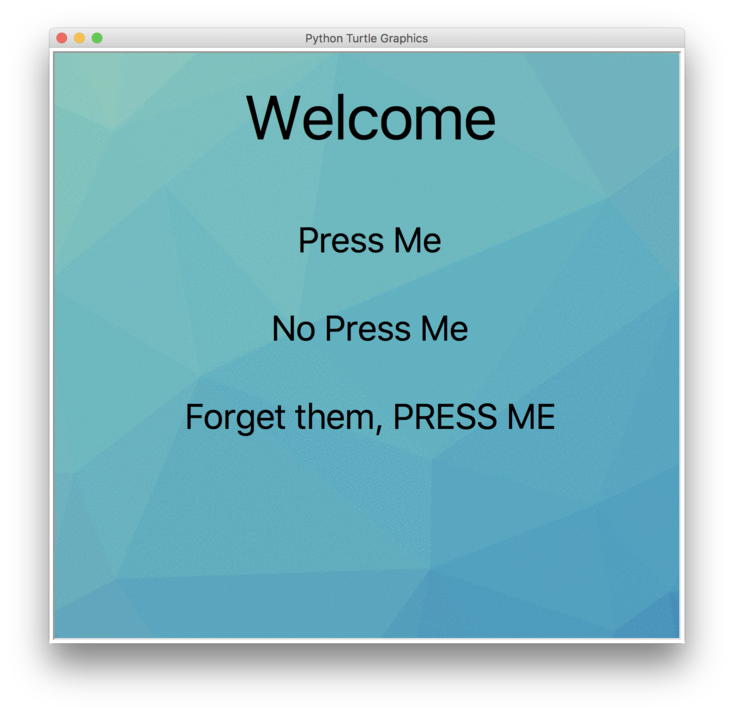
\includegraphics[width=4cm]{Menu_2}
}\hspace*{-1.5cm}

This looks good. Lets now add a border \ldots 

\subsubsection{Draw the border}

\TODO{After the  ``\code{draw border}'' comment insert code that draws a 
rectangle of width \code{w}, and height \code{h}}

\codeonly{title={\code{Menu.py}}}{40}{45}{code}{Menu_3.py}  
\mbox{}\hfill\raisebox{0.5cm}[0pt][0pt]{%
	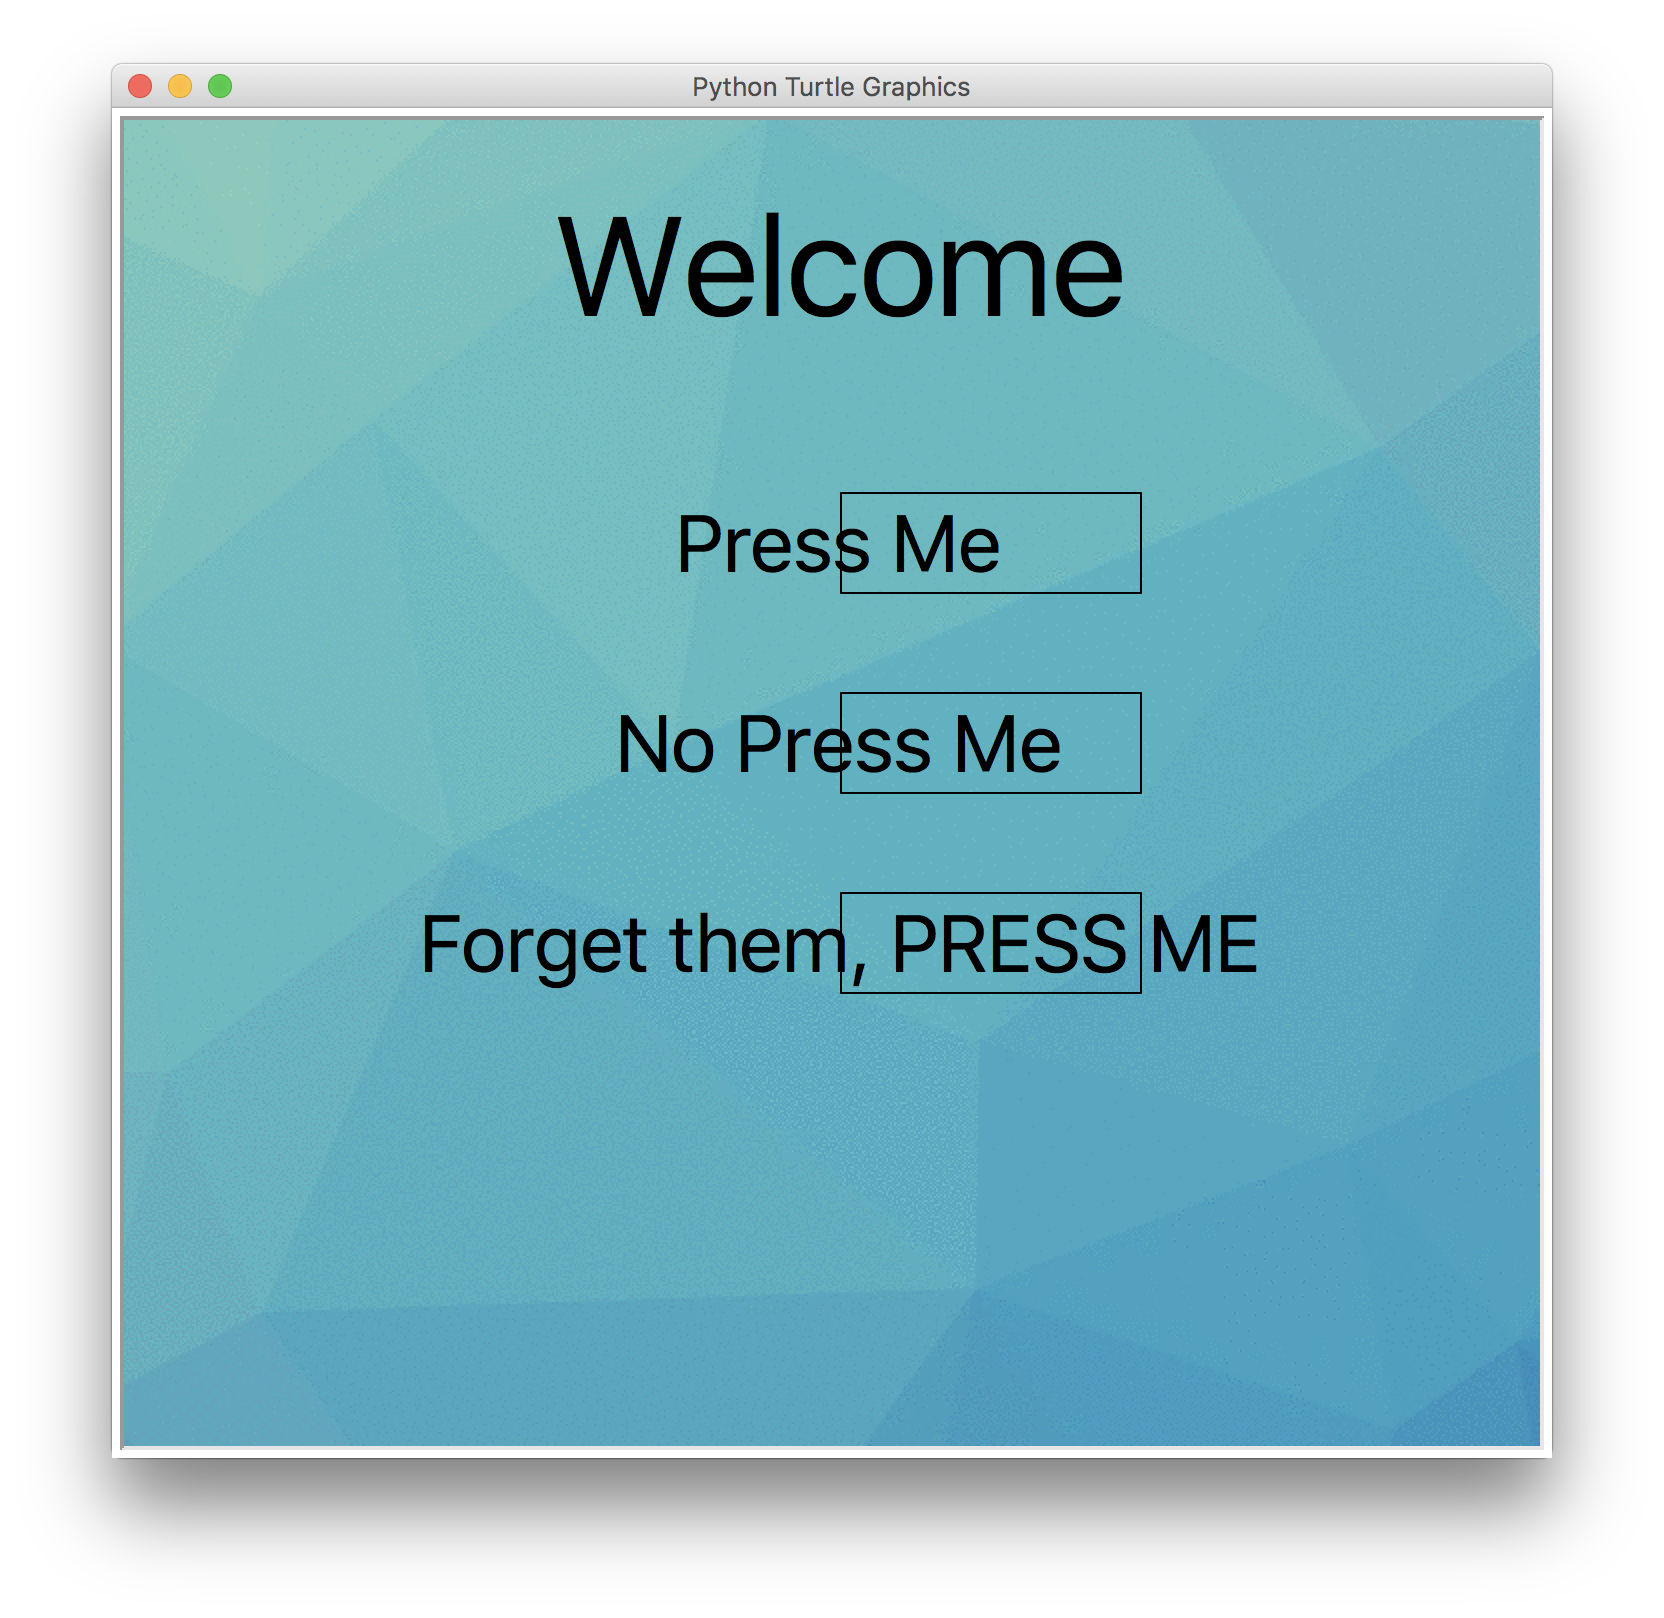
\includegraphics[width=4cm]{Menu_3}
}\hspace*{-1.5cm}

I see two problems here. The width of the rectangles is too small --- this is easy to fix. We just set the \code{w} parameter when calling \code{drawButton}. The second problem is that the rectangle is drawn starting from the bottom centre of the label --- we fix this by moving \code{bob} to the bottom left corner (see Figure~\ref{fig:button}).

\TODO{Insert code to move \code{bob} to bottom left corner, and change the widths of the 
button in your \code{drawButton} calls by setting parameter \code{w}. You should then get the following.}

\codeonly{title={\code{Menu.py}}}{40}{46}{code}{Menu_4.py}  
\mbox{}\hfill\raisebox{0.5cm}[0pt][0pt]{%
	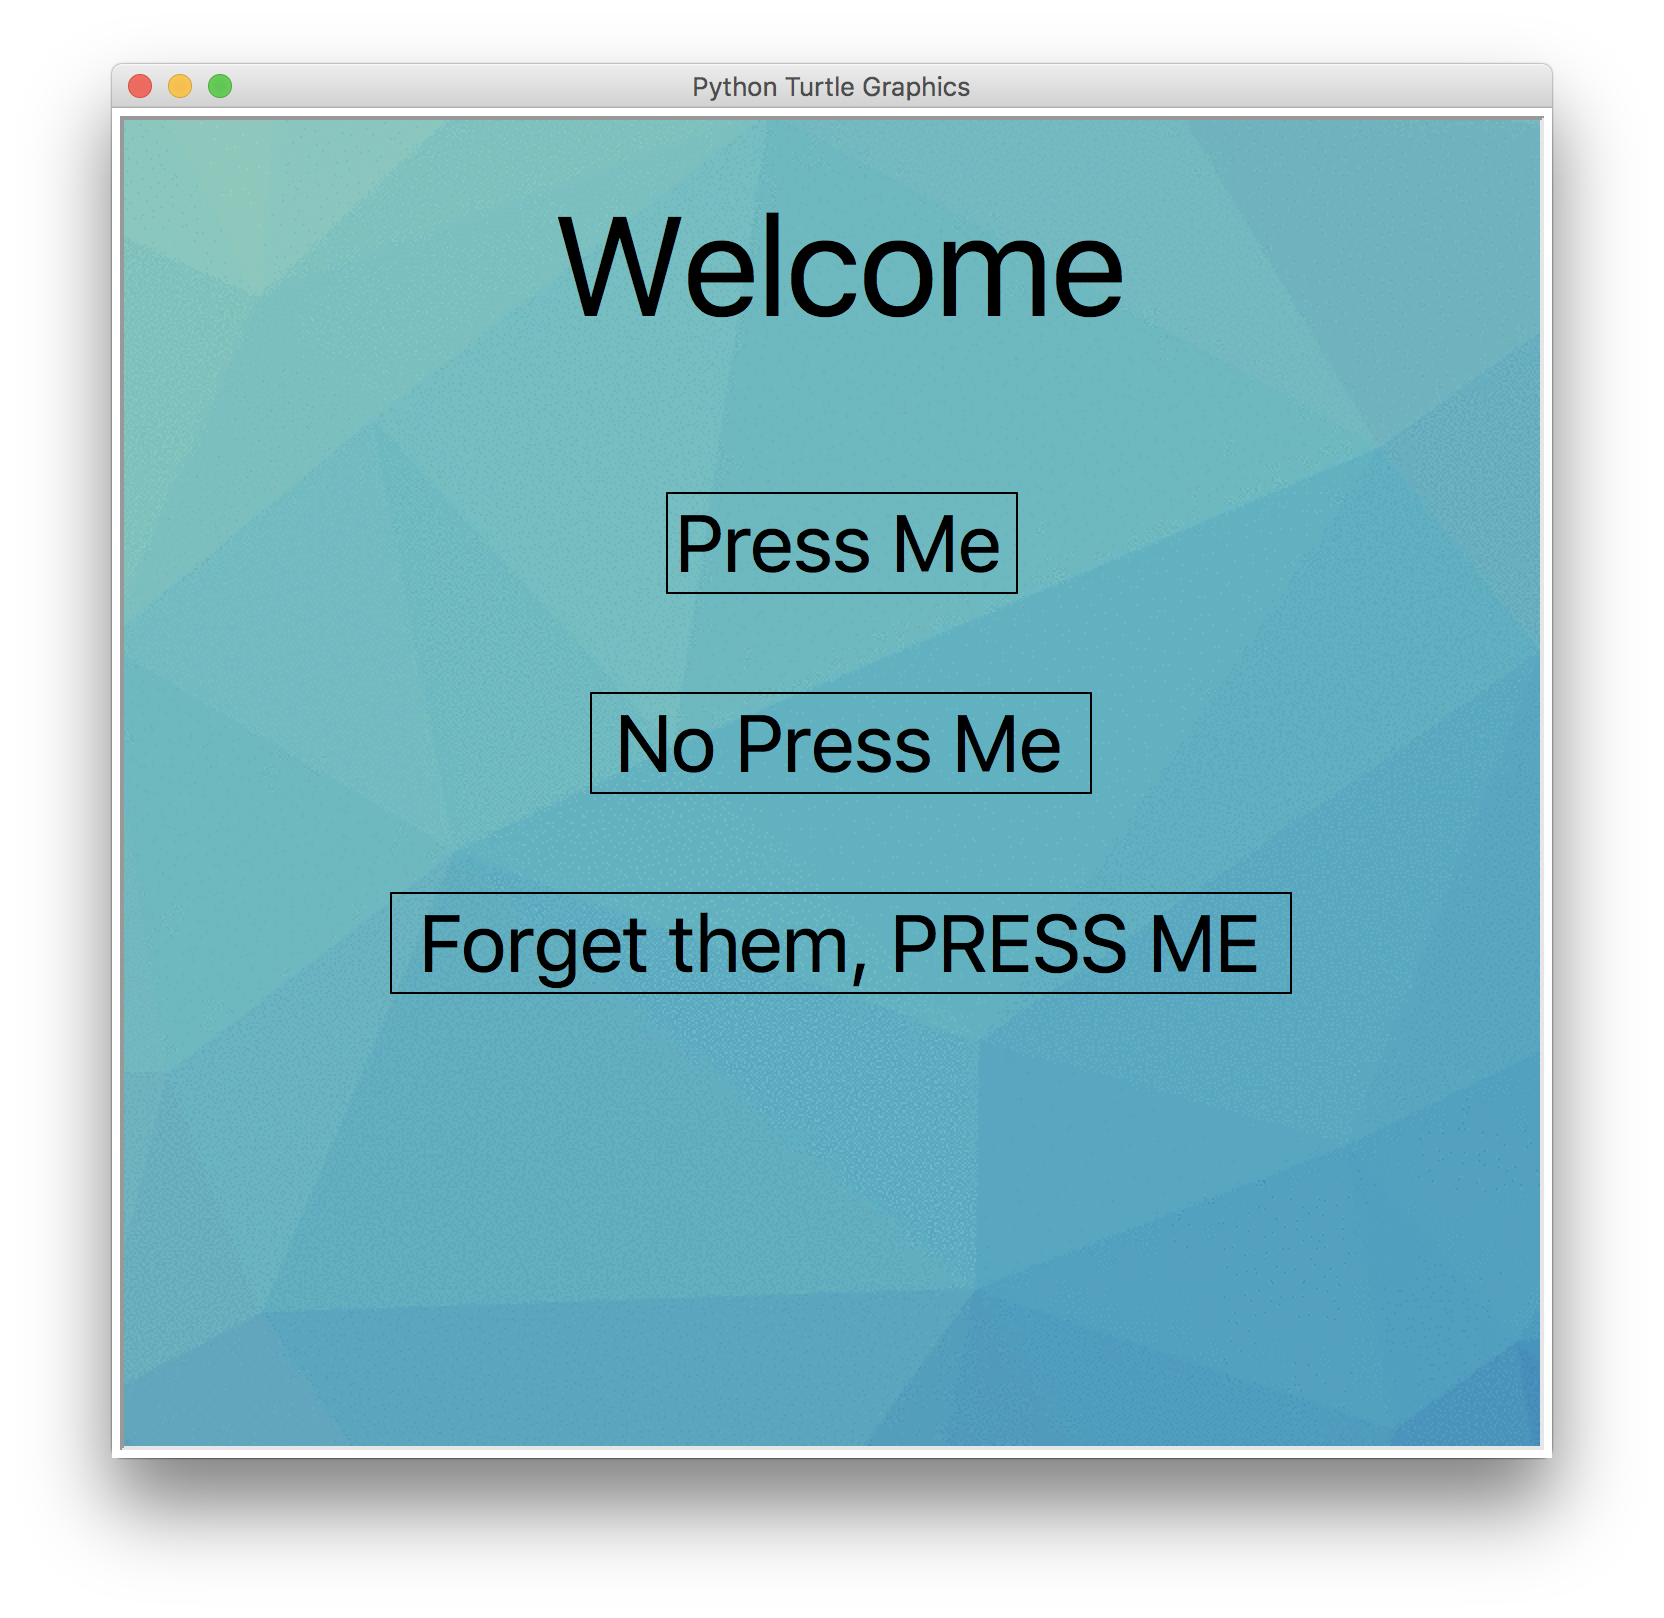
\includegraphics[width=4cm]{Menu_4}
}\hspace*{-1.5cm}

Now the above works, but putting basic drawing of a rectangle inside our draw button is not a great idea.  We will be drawing lots of rectangles so lets move that code out into a new helper function.

\TODO{Before your \code{drawButton} function in \code{Define helper functions} section, insert the following function}

\codeonly{title={\code{Menu.py}}}{31}{46}{code}{Menu_5.py}  

This function will draw a rectangle of width \code{w}, and height \code{h}, with bottom left corner at position (\code{x},\code{y}). You can also specify the border colour and the fill colour.

\vspace{12pt}

You should think about extending this function by, for example,
\begin{itemize}
\item Adding parameter \code{pensize=2} which would set the thickness of the border.
\item Adding parameter \code{shadow=False} which when set to \code{True} would draw a shadow. 

Drawing a shadow, is actual easy --- we just draw a few rectangles a little to the right an a little below the position of the main rectangle BEFORE we draw the main rectangle. If you are exceedingly lazy (this is a good thing in a programmer!) you can draw the shadow rectangles by just calling the \code{drawRectangle} function from inside the  \code{drawRectangle}
\end{itemize}
\newpage

Now your \code{drawButton can be simplified to}

\codeonly{title={\code{Menu.py}}}{49}{59}{code}{Menu_5.py}
\mbox{}\hfill\raisebox{0.85cm}[0pt][0pt]{%
	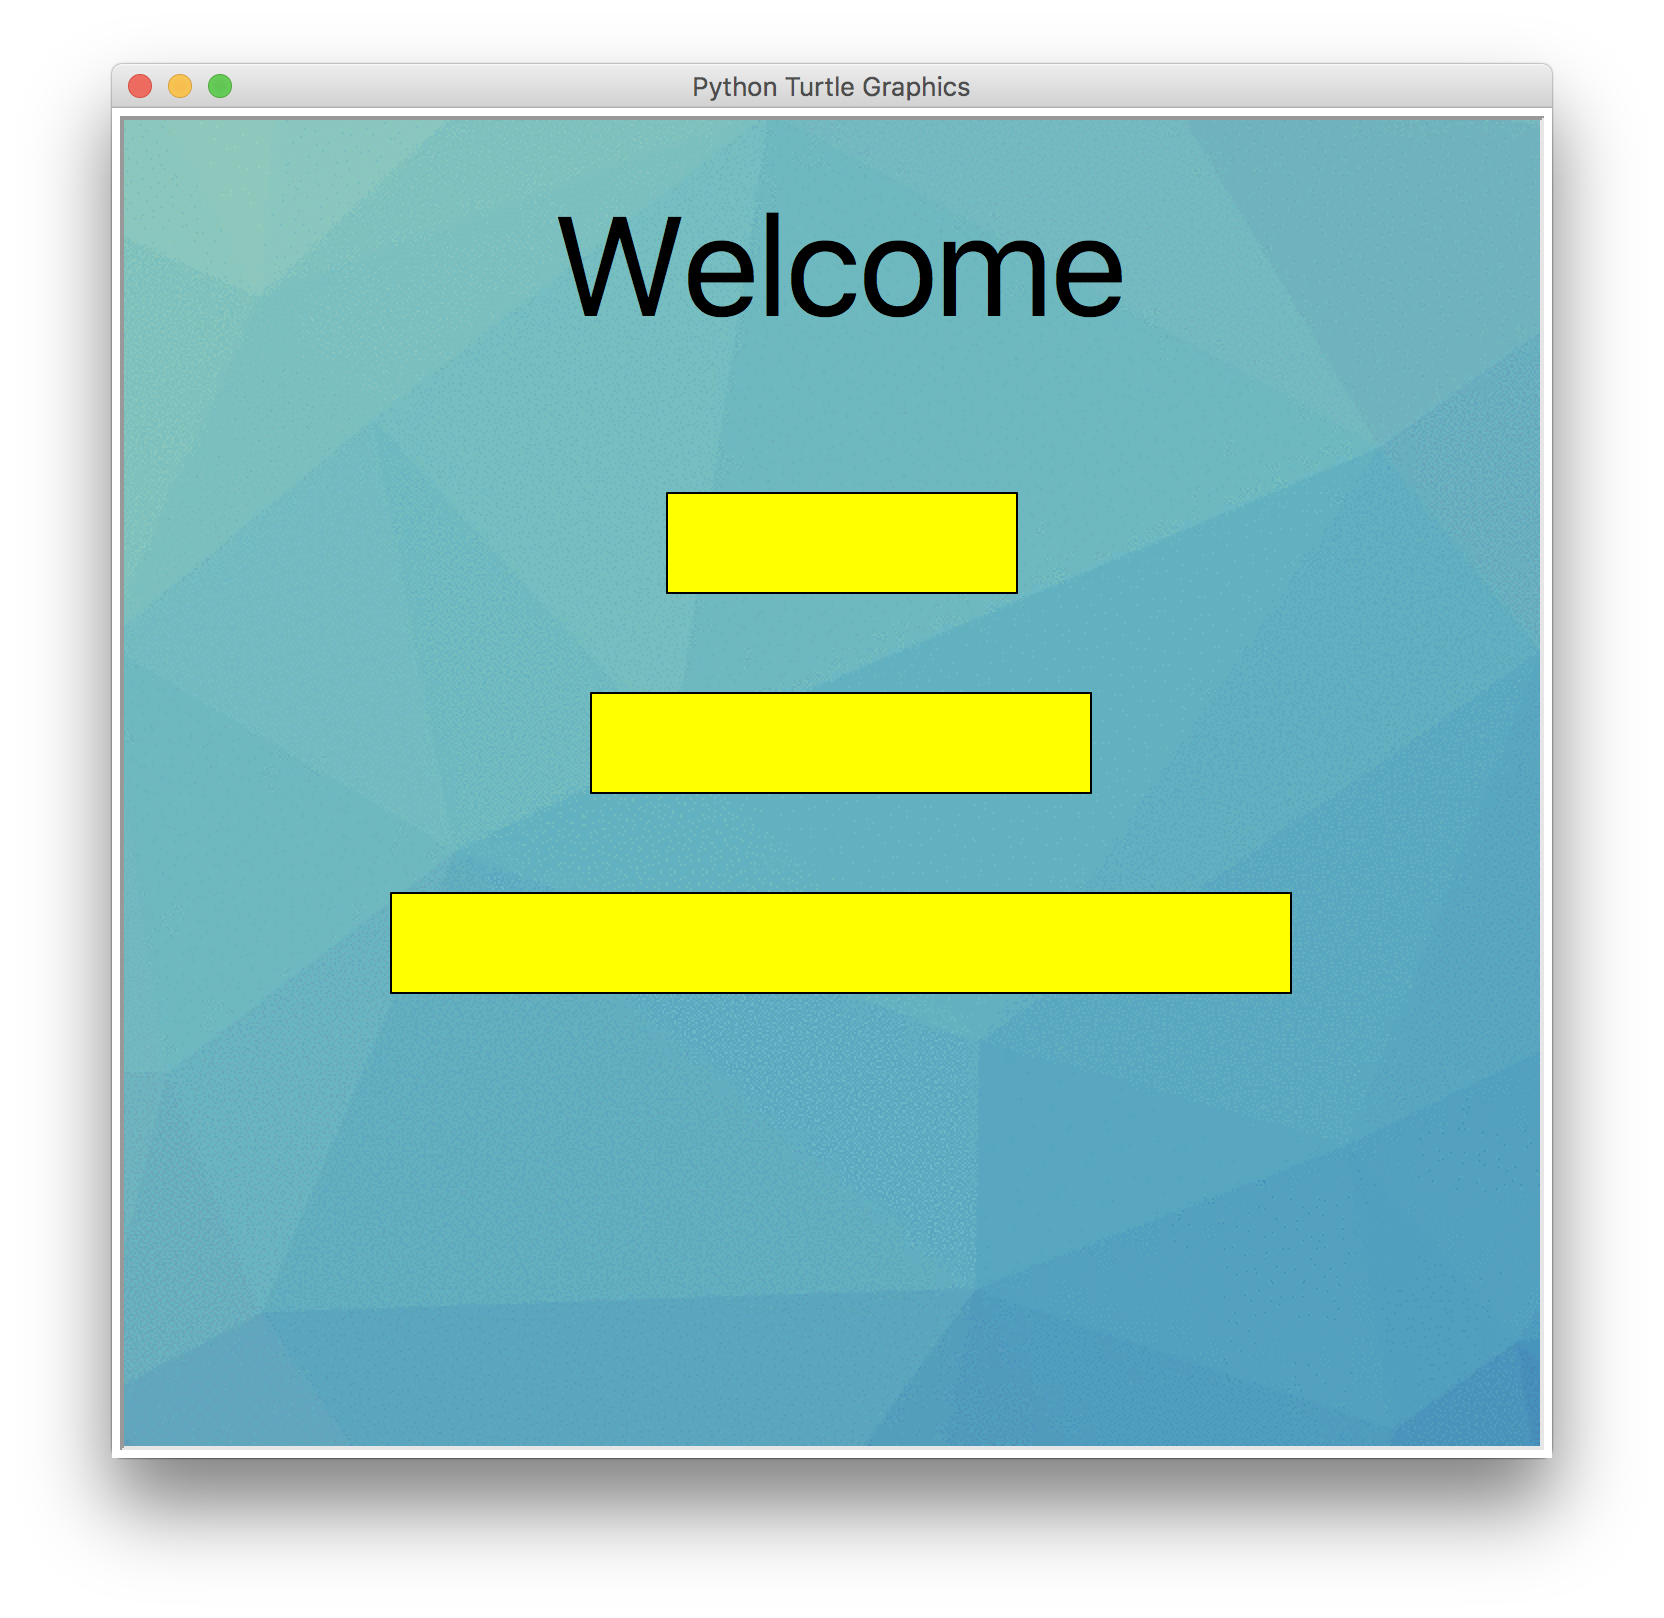
\includegraphics[width=4cm]{Menu_5}
}\hspace*{-1.5cm}

\TODO{If you look, really really carefully at the output you will see that {\em we} have done something silly.  To fix this, we need to draw the button label after drawing the border. Fix This.}

\codeonly{title={\code{Menu.py}}}{54}{64}{code}{Menu_6.py}
\mbox{}\hfill\raisebox{0.85cm}[0pt][0pt]{%
	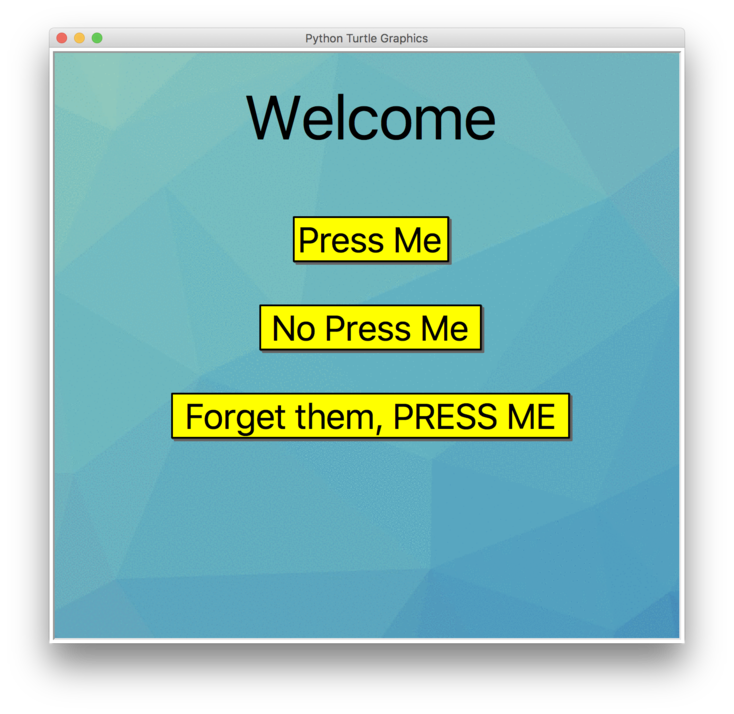
\includegraphics[width=4cm]{Menu_6}
}\hspace*{-1.5cm}


\subsubsection{Making the buttons work}

OK, now we have things that looks like buttons, but they do not act like them --- click on a button and see what happens --- nothing. 

To get the buttons to work we need to do two things:

\begin{itemize}
\item Listen for and respond to click events.

This is easy --- we will create our own \code{onclick} function to run whenever the user clicks on the screen.

\item When a click occurs, decide whether it happened within a button region and which button.

This is a little harder so we will talk about this in some detail.
\end{itemize}

\newpage

\TODO{Insert the following function at the bottom of the ``\code{Define helper functions}'' section of your code.}

\codeonly{title={\code{Menu.py}}}{67}{69}{code}{Menu_7.py}

and just before the \code{turtle.mainloop()} insert the lines

\codeonly{title={\code{Menu.py}}}{84}{85}{code}{Menu_7.py}

Now run your code and make sure you see a message appearing in {\em Thonny} every time you click the left mouse button. You should see that you also get the position of the mouse in the screen when the click occurred. Next we need to use this position information to determine which button was ``pressed''.

\TODO{Insert the code at the bottom of the ``\code{Create screen}'' section of your code.}

\codeonly{title={\code{Menu.py}}}{21}{23}{code}{Menu_8.py}

\begin{itemize}
\item
Lines 21 and 22, allow us to create an object (like the \code{Turtle} object or the \code{Screen} object) which stores information for a Button. Our \code{Button} object stores position (\code{x},\code{y}), size  \code{w} by \code{h}, and \code{label}.
\item
Line 23 defines an empty list, called \code{buttons}, that will store the information for all generated buttons.
\end{itemize}

So where do we get the information that we want to store in the \code{buttons} list?  

We have this information at end of \code{drawButton} function so that is where we will build our \code{Button} object.

\TODO{Modify the \code{drawButton} function so that it returns a \code{Button} object, as shown below.}
 
\codeonly{title={\code{Menu.py}}}{58}{69}{code}{Menu_8.py}

Now \code{bob} has a list of all of the generated buttons which we can search whenever the user clicks on the screen. First we need to make sure we are happy with our geometry. The mouse click is recorded at the point (\code{mx},\code{my}).  The conditions that must be true if this point is inside a button rectangle are shown in the following figure.

\begin{figure}[H]
\centering\larger[2]\vspace{-18pt}
\begin{tikzpicture}
	\draw[dashed,fill=yellow!20] (-5,0) rectangle (5,1.5);
	\fill[red] (0,0) circle (.1) node[below,black] {(\code{x},\code{y})};
	
	%\node[font={\larger[4]}]  at (0,0.75) {Press Me!};
	\draw[|-|] (5.5,0) -- node[fill=white] {\code{h}} ++(0,1.5); 
	\draw[|-|] (-5,1.8) -- node[fill=white] {\code{w}} ++(10,0); 
	\fill[blue] (-5,0) circle (.1) node[below,left,yshift=-9pt] 
	{(\code{x}-\code{w/2},\code{y})};
	\fill[blue] (5,1.5) circle (.1) node[above,right,yshift=12pt] {(\code{x+w/2},\code{y+h})};
	
	\fill[green!80!black] (3,1) circle (.1) node[below left,black] {(\code{mx},\code{my})};
	
	\draw[decorate,decoration={brace,amplitude=10pt}] (5,-1) -- 
	node[below, yshift=-15pt,fill=white,draw,drop shadow] 
	{\code{x}-\code{w/2 < mx <  x+w/2}}
	++(-10,0);

	\draw[decorate,decoration={brace,amplitude=10pt}] (-5.5,0) -- 
	node[left, xshift=-15pt, fill=white,draw,drop shadow] 
	{\code{y < my <  y+h}}
	++(0,1.5);
	
\end{tikzpicture}
\caption[Given button and point, determine if point is inside button]{Given a button and a point (\code{mx},\code{my}), determine if point is inside button.\label{fig:button}}
\end{figure}

\TODO{Modify your \code{onclick} function so that it check every button stored in \code{bob.buttons} using the conditions on (\code{mx},\code{my}) shown in the above figure.\\

Run this code and verify that whenever you click on a button that button's label is printed.
}

\codeonly{title={\code{Menu.py}}}{72}{78}{code}{Menu_8.py}


So finally we want to run different code depending on which button has been pressed. To do this we check the label of the button.

\TODO{Update the \code{onclick} function as shown below.}

\codeonly{title={\code{Menu.py}}}{72}{87}{code}{Menu_9.py}

\subsection{It's Lego time --- Putting your Programs Together}

OK, we now have nearly everything to build our menu. To get the menu layout that I showed at the start of this worksheet I used the following code.  You don't have to follow this.

\codeonly{title={\code{Menu.py}}}{99}{118}{code}{Menu_10.py}
\mbox{}\hfill\raisebox{7cm}[0pt][0pt]{%
	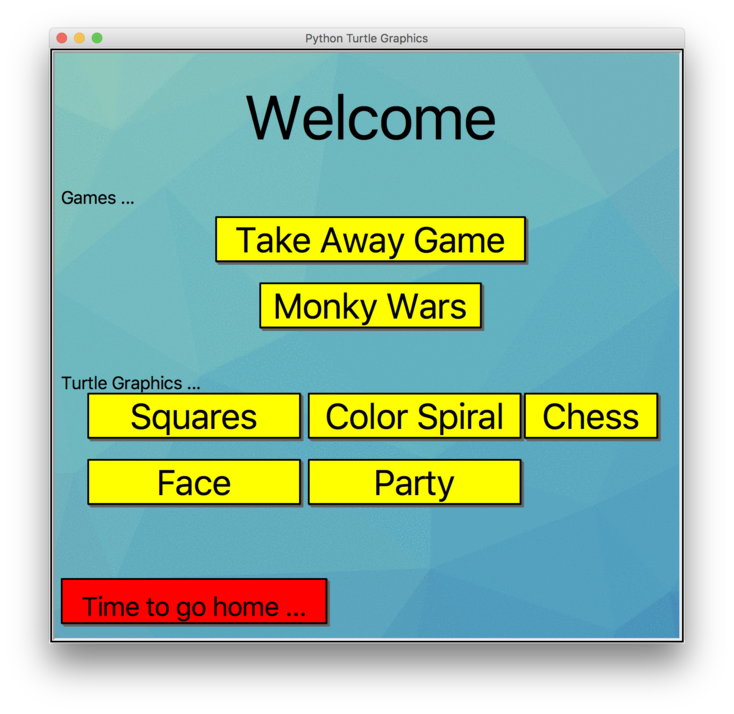
\includegraphics[width=6cm]{Menu_Complete}
}\hspace*{-1.5cm}

Then in my \code{onclick} functions I have added {\bf some} of the code needed to respond to the above button clicks.
 
\codeonly{title={\code{Menu.py}}}{72}{89}{code}{Menu_10.py}

Notice in line 80 and in line 83 I run other python files.  You will need to change this to match the name that you used for your files.
\end{document}




